\chapter[The Standard Model]{The Standard Model and beyond}
\label{chap:SM}
Since the Greeks, different theories about the composition and structure of the world have been formulated. At ancient Greece these theories were elaborated from a philosophical point of view. Nowadays, a very sophisticated set of tools and concepts has been developed, this allowed the construction of a general vision of nature, its components and structure. Moreover, on the subject of the constituents, or elemental constituents, a theory capable of describing the majority of known phenomena has been developed. This theory is the Standard Model (SM) of particle physics. It is a model constructed by the contribution of many people. One of its seminal papers is~\cite{PhysRevLett.19.1264}. A modern formulation of this model is presented in~\cite{Griffiths:2008zz}. 

This SM relies on two of the more elegant constructs of modern physics and mathematics. From the physics side, the quantum field theory; from mathematics, group theory. Quantum field theory~\cite{RevModPhys.13.203} has born from the understanding of processes that take place at very small spatial scales and in a regime where special relativity plays an important role. To describe such, a major part of the most brilliant minds of the 20th century dedicated their life, Paul Dirac~\cite{Dirac:1927dy}, Richard Feynman~\cite{Feynman:1950ir}, Enrico Fermi~\cite{Fermi:1934hr} among them. The theory of quantum fields has set in a common place two extraordinary achievements of physics: special relativity~\cite{Einstein:1905ve} and quantum mechanics. With it many phenomena have been described: $\beta$ and $\alpha$ decay, solid state, among many other.

From the mathematics side, group theory has become one of the most powerful tools for particle physicist. A modern presentation of this theory, oriented to particle physics, is done in~\cite{Georgi:1999wka}. However, its development began quite early, with Galois around 1830~\cite{Galois:2013}, and was used in other parts of physics, it is with Lie algebras~\cite{Georgi:1999wka} and the possibility of describing continuous symmetries that the most important step were given. Also, this would have not been possible without the amazing connection found by Emmy Noether in 1918~\cite{1971TTSP....1..186N}. She found that for every conserved quantity there is a preserved symmetry. Group theory can be seen, roughly speaking, a way to mathematically describe symmetries, group theory became the tool to describe systems with conserved quantities. 

In this chapter, the basics of the SM are presented. Its seminal ideas are presented, its structure and content and its ultimate consequences. Also its limitations are discussed and how a new theory addresses part of them. The chapter finishes with the description of the production of some of SM particles in the Large Hadron Collider~\cite{1748-0221-3-08-S08001}. 

\section{Fields, symmetries and interactions}
\label{sec:symm}

From the very beginning of physics, one of the most fundamental questions has been how does bodies interact, and what is exactly an interaction. On the first type of interaction ever studied by physics, gravity, Newton proposed the concept of distant interaction~\cite{Newton:2014}, the idea that bodies could interact without being in direct contact. But the question on how exactly that distant action was performed remained unanswered. 

During the 19th and 20th century new phenomena were discovered pointing to brand new interactions, electricity, magnetism and radioactivity~\cite{Pauli:1930pc}. The very precise and complete description of electromagnetism developed by Gauss, Faraday, Amp\`{e}re and finished by Maxwell succeeded to describe electricity and magnetism under the formalism of only one interaction within the mathematical formalism of classical fields. Further works addressed radioactivity, driving to a deeper understanding of nature and its composition.

%For the following discussion, and later, we are going to work in natural units for simplicity. In these units the speed of light $c$ is normalized to unity, as well as electron electric charge $e$, reduced Planck constant $\hslash$ and Boltzmann constant $k_{B}$. Then, masses and temperature are expressed in energy units, i.e. $eV$, and time and length in inverse energy units, $eV^{-1}$.

A classical field is an assignment of a quantity to every point in space and time. For physics, the quantity that is attributed is a physical quantity such as mass, electrical charge or momentum. This quantity can be scalar or vector, giving rise to the notion of scalar or vector field, correspondingly. A comprehensive study of this concepts is done in~\cite{Feynman:2013}. The simplest example, is the temperature in a gas, that is a scalar quantity assigned to every point. Another example, a fluid can be described in terms of fields, being its velocity a vector field and its pressure a scalar field. Generic classical electromagnetic interactions can be described with the help of one vector field $\vec{A}(x)$, the vector potential, and one scalar field $\phi(x)$, the scalar potential. In Einstein's special relativity~\cite{Einstein:1905ve}, dynamics of physical objects are described via the formalism of four vectors. In Newtonian dynamics~\cite{Goldstein:2001} the position or speed of an object are described in three dimensional space by a three dimensional vector. In relativistic dynamics, one dimension is added to these vectors, for example the three dimensional position vector has an additional temporal dimension, or the momentum vector has an additional dimension with the energy of the object. In this formalism the scalar and vector potential can be organized in the four-potential $A_{\mu}=(-\phi,\vec{A})$. This can be used to define the strength field tensor $F_{\mu\nu}=\partial_{\mu}A_{\nu}-\partial_{\nu}A_{\mu}$, where $\partial_{\mu}=\left( -\frac{\partial}{\partial t},\nabla\right)$ is the covariant derivative. From this tensor it is possible to obtain in a very generic and elegant way the equations of motion of the free field using the Lagrangian formalism, as in equation~\ref{eq:electromotion}. With the Lagrangian density defined in equation~\ref{eq:electrolagran}. The Lagrangian formalism is a generalization of Newtonian dynamics that allows to obtain from a generic principle the equations of motion of a system. This formalism is described in~\cite{Maggiore:2005qv}. 

\begin{equation}
  \label{eq:electromotion}
  \partial_{\mu}\left( \frac{\partial \mathcal{L}}{\partial (\partial_{\mu}A_{\nu})} \right) -\frac{\partial \mathcal{L}}{\partial A_{\nu}}=0
\end{equation}

\begin{equation}
  \label{eq:electrolagran}
  \mathcal{L}=-\frac{1}{4}F^{\mu\nu}F_{\mu\nu}
\end{equation}

It is very important to notice that the equations of motion of the free field are invariant under the choice of the four-potential. More precisely, the covariant potential is not unique and the covariant derivative of a scalar field, $\partial_{\mu}\Lambda(x)$, can always been added, 
\begin{equation}
  \label{eq:gaugeA}
  {A'}_{\mu}=A_{\mu}+\partial_{\mu}\Lambda(x) \leftrightarrow \partial^{\mu}A_{\mu}=0
\end{equation} and describe the same physics. This non-uniqueness corresponds to the choice of a zero-point of the potential very well known in non-Lagrangian formalism of electrodynamics. When a specific value for this scalar field is chosen, $\Lambda(x)$, it is said that the gauge has been fixed. Further details are given in~\cite{Jackson:1998nia}.

A four current vector can also be defined, $J_{\mu}=\left( \rho,\vec{J} \right)$ with $\rho$ the electric charge density and $\vec{J}$ the current charge density. Then, plugging in this four current in the Lagrangian of the free field, defined in equation~\ref{eq:electrolagran}, 

\begin{equation}
  \label{eq:fulleleclagrangian}
  \mathcal{L}=-\frac{1}{4}F^{\mu\nu}F_{\mu\nu}-A_{\mu}J^{\mu}
\end{equation}the complete set of equations of motion of the field with charges and currents are obtained.

The transformation stated from equation~\ref{eq:gaugeA} can be understood as a transformation of the field. These type of transformations are mathematically understood under the group $U(1)$~\cite{Georgi:1999wka}, where the generic transformation operator can be written as $U=e^{i\theta(x)}$. It is said then that the electromagnetic vector potential is invariant under $U(1)$ transformations. This property identifies an essential characteristic of electromagnetism, its symmetric behavior under $U(1)$. 

From this reasoning the most interesting results are drawn when the same symmetry is imposed to other fields. For example, the kinetic Lagrangian for a complex scalar field is $\mathcal{L}=(\partial^{\mu}\phi)^{*}\partial_{\mu}\phi$. To perform the transformation on the scalar field, it is sufficient to apply the operator as $\phi'=U\phi$ and ${\phi'}^{*}={\phi}^{*} U^{-1}$. But it is evident that the Lagrangian is not the same after applying such transformation. Then, in order to preserve the Lagrangian under $U(1)$ it is necessary to change at the same time the derivative. Such transformation is given in equation~\ref{eq:covderivU1}, where $g$ is a constant.

\begin{equation}
  \label{eq:covderivU1}
  \mathcal{D}^{\mu}=\partial^{\mu}-igA^{\mu}
\end{equation}

Then, the proposed Lagrangian can be rewritten, including the vector field, as

\begin{equation}
  \label{eq:FullLagU1inv}
  \mathcal{L}=(\mathcal{D}^{\mu}\phi)^{*}\mathcal{D}_{\mu}\phi-\frac{1}{4}F^{\mu\nu}F_{\mu\nu}
\end{equation}which is invariant under $U(1)$. An interaction term, of the form $igA^{\mu}\phi^{*}\partial_{\mu}$, between the scalar and the vector field, can be derived from the kinematic part of the Lagrangian~$(\mathcal{D}^{\mu}\phi)^{*}\mathcal{D}_{\mu}\phi$. This shows that the requirement of the invariance under $U(1)$ of the scalar field leads to the introduction of an interaction with a vector field controlled by the constant $g$. The electromagnetic interaction is described precisely by a vector field and preserves $U(1)$ symmetry, which implies that this symmetry is the connection to electromagnetic interaction, identifying the interaction itself with the $U(1)$ symmetry. In addition, using Noether theorem~\cite{1971TTSP....1..186N} it can be shown that $g$ is a conserved quantity, as the electric charge is.

But not only electromagnetism can be described via a continuous symmetry as $U(1)$. On 1896 radioactivity was discovered by the french physicist Henri Becquerel~\cite{Becquerel:1896zz}. Three years after, Marie and Pierre Curie~\cite{Curie:1898} studied in more detail the phenomenon and found Polonium and Radium elements. And later on, Ernst Rutherford~\cite{Rutherford:1911zz} was able to describe radioactivity as coming in three types, alpha ($\alpha$), beta ($\beta$) and gamma ($\gamma$). He also noticed that radioactivity was able to change matter, which allowed him, with also other experiences, to propose an atomic model, describing elements as basically and external core of negative charges and a nucleus positively charged. Consequently, this findings implied the existence of interactions different to electromagnetism, acting at the atomic scale.

The interaction that undergoes radioactivity, beta decay, is called the weak interaction. In 1934 Enrico Fermi made a first theoretical description of this interaction~\cite{Fermi:1934hr}, but only in 1968 Sheldon Glashow, Abdus Salam and Steven Weinberg were able to describe the weak interaction with a symmetry group: $SU(2)$~\cite{Glashow:1967rx, Salam:1968rm}. Finally, the interaction that keeps the nucleus components together, the strong interaction, was described with $SU(3)$ group mainly by Murray Gell-Mann in 1964~\cite{GellMann:1964nj}.

There have been many attempts to describe gravity with the same formalism, but up to present such attempts have been unsuccessful. Such question remains one of the most important problems for modern particle physics.  

\section{Quantum fields and particles}
\label{sec:fields}

Classical fields, introduced and described in last section~\ref{sec:symm}, can be extended to a quantum theory. Such procedure is known as the quantization of fields and allows to unify special relativity and quantum mechanics in one theory, Quantum Field Theory (QFT). It describes the dynamics of systems in the regime where the speed is close to the speed of light in the atomic or smaller scales.

Quantum mechanics introduced two fundamental concepts: first, the description of the system by its states; and second, the identification of an observable with an operator. The state of a system is identified with a set of quantum numbers that characterizes the system state. For example, the energy is a quantum number of the hydrogen atom system, such that each state has a value for the energy related the potential energy contained in the system. Quantum states are mathematically noted in Dirac notation as a ket,

\begin{equation}
  \label{eq:DiracNot}
  \ket{\alpha}=\ket{i,j,k,\dots}
\end{equation}with $\alpha$ the set of quantum numbers $i,j,k,\dots$ This mathematical object lives in Hilbert space (a complex space $\mathds{C}$ of functions), the conjugate of which, a bra, is noted $\bra{\alpha}$, and their internal product $\braket{\beta}{\alpha}$. The numerical value of $|\braket{\beta}{\alpha}|^{2}$ gives the transition probability of the system from state $\beta$ to state $\alpha$, and $|\braket{\alpha}{\alpha}|^{2}$ is the probability to find the system in the state $\alpha$.

Physical observables like position, energy or momentum are described by complex operators such that in order to measure their value for a given state, $|\bra{\alpha}\hat{O}\ket{\alpha}|^{2}$ has to be calculated. The identification of observables and operators is called first quantization. In addition, the Schr\"{o}dinger equation~\cite{ANDP:ANDP19263840404} describes the evolution of states,

\begin{equation}
  \label{eq:Schrodinger}
  \hat{\mathcal{H}}\ket{\alpha}=i\frac{d}{dt}\ket{\alpha}
\end{equation}with $\mathcal{H}$ the Hamiltonian of the system. The whole formalism is able to explain quantized systems, where the quantum numbers are discrete, such as hydrogen atom or black body.

Several functions or fields can be related to a system. These functions, wave functions, can be used to calculate the probability of a system to be in a given state or the transition probability between states. In second quantization, wave functions are upgraded into field operators. This procedure gives rise to the quantization of the state of the field, which is described by the quantum number $n$ which is definite positive: $n=0$ for the fundamental state and $n>0$ for the excited states. Such excitations of the field are understood as physical particles, or quanta, that propagate in space-time, which means that $n=0$ is vacuum. 

The first QFT ever created was born from the quantization of the electromagnetic field. Quantum Electro Dynamics (QED) is the quantized version of classical electrodynamics, that was developed by Tomonaga, Schwinger and Feynman around 1940~\cite{Tomonaga:1948zz, Schwinger:1948yk, Feynman:1948ur}. This theory describes electromagnetic interactions of a charged field and the electromagnetic vector field. The charged field excitations correspond to electrons and the excitations of the vector fields are photons, responsible of light. Electrons are particles with negative electric charge that orbits around the nucleus in atoms. Discovered in 1897 by J. J. Thomson~\cite{Thomson:1897cm}, it was fully described by P. A. Dirac in 1927~\cite{Dirac:1927dy} with the Dirac equation that is the Schr\"{o}dinger equation for a relativistic particle of spin 1/2. Spin, the intrinsic angular momentum carried by a particle, can be integer (0,1,2,...) or semi-integer ($\frac{1}{2}$,$\frac{3}{2}$,...). The particles with semi-integer spin, as electrons, are called fermions and particles with integer spin, as photons, are called bosons. Dirac equation predicted the existence of a particle identical to the electron but with positive charge, the positron. It was discovered in 1931 by Carl David Anderson~\cite{Anderson:1933mb}.

The SM has three fundamental interactions: electromagnetic, weak and strong interactions. Each fundamental interaction has associated a charge. Charged particles interact via the corresponding force. The electromagnetic interaction has associated electric charge. The weak charge is called the weak isospin. Finally, the strong force charge is the color.

Up to present days 12 fundamental fermions and 5 fundamental bosons have been found. Fermions are organized in leptons, that do not interact strongly, and quarks, that do interact strongly. Leptons are organized in three families, the electron ($e^{-}$) and electron neutrino ($\nu_{e}$), muon ($\mu^{-}$) and muon neutrino ($\nu_{\mu}$) and tau ($\tau$) and tau neutrino ($\nu_{\tau}$). Electron, muon and tau are electrically charged while neutrinos are neutral. Their respective anti-particles are equally organized, positron ($e^{+}$) with electron anti-neutrino ($\bar{\nu}_{e}$), anti-muon ($\mu^{+}$) with muon anti-neutrino ($\bar{\nu}_{\mu}$) and anti-tau ($\tau^{+}$) with tau anti-neutrino ($\bar{\nu}_{\tau}$). Quarks also come in three families, with the respective anti-quarks: up ($u$, $\bar{u}$) and down ($d$, $\bar{d}$), charm ($c$, $\bar{c}$) and strange ($s$, $\bar{s}$), top ($t$, $\bar{t}$) and bottom ($b$, $\bar{b}$). The fundamental bosons are the photon ($\gamma$), the \W~(positively and negatively charged) and \Z~that mediate the electroweak interaction, the gluons ($g$) mediating the strong interaction and the Higgs (\Hb). The Higgs boson does not mediate an interaction but plays another role in the SM, that will be described in section~\ref{sec:mass}. The strong force mediator, the gluon, was discovered by the PETRA~\cite{Brandelik:1979bd} and PLUTO~\cite{Berger:1979cj} experiments in 1979 at DESY. The weak bosons were discovered at CERN in 1983 by the UA1 and UA2 collaborations~\cite{Hansen:1984mw} at the SPS accelerator~\cite{SPS:REF} (described on section~\ref{sec:injector}), called at that time Sp$\bar{\text{p}}$S because it was a proton-antiproton collider. The Higgs boson has been discovered recently in 2012 by ATLAS~\cite{1748-0221-3-08-S08003} and CMS~\cite{1748-0221-3-08-S08004} experiments at the LHC~\cite{Aad:2012tfa, Chatrchyan:2012xdj}. The 2013 physics Nobel prize~\cite{Nobel2013} was awarded to Francois Englert and Peter W. Higgs "for the theoretical discovery of a mechanism that contributes to our understanding of the origin of mass of subatomic particles, and which recently was confirmed through the discovery of the predicted fundamental particle, by the ATLAS and CMS experiments at CERN's Large Hadron Collider". The particle content of the SM is resumed in figure~\ref{fig:SMContent}.

\begin{figure}[!Hhtbp]
  \begin{center}
    \includegraphics[width=0.7\textwidth]{figs/Standard_Model_of_Elementary_Particles.jpg}
    \caption{Particle content of the standard model.}
    \label{fig:SMContent}
  \end{center}
\end{figure}

In the next section one of the fundamental pieces of the SM is going to be described: how particles acquire mass. Whatsoever, even if the mechanism to give mass to particles is one of the most refined theoretical constructs, it leaves some unsolved puzzles in the heart of the SM. Later, the limitations of the SM and some theoretical insights to solve them are discussed.

\section{The mass problem}
\label{sec:mass}

Using the concepts developed on previous sections about QFT and symmetries it is possible to construct a whole theory giving rise to a precise description of particles and interactions between them. But such a theory does not allow to have massive bosons, whereas masses for fermions are allowed. A mass term for a fermion $\psi$ is of the form 

\begin{equation*}
%  \label{eq:elemass}
  m_{\psi}\bar{\psi}\psi
\end{equation*} where $m_{\psi}$ is the mass of the field.

Under $U(1)$ transformations, $\psi'=U \psi$, the mass term remains the same, which means that it is invariant under $U(1)$ transformations. The same is not true for a boson. A mass term for a boson $A$, can be written as 

\begin{equation}
  \label{eq:Amass}
  m_{A}A^{\mu}A_{\mu}
\end{equation} where $m_{A}$ is its mass.

The $U(1)$ transformation for the boson is $A'^{\mu}=A^{\mu}+\delta^{\mu}\theta(x)$, where $\delta^{\mu}\theta(x)$ represents an infinitesimal variation of the field by the coordinate depending parameter $\theta(x)$. Applying such transformation on the mass term~\ref{eq:Amass}, the transformed term can be obtained

\begin{equation}
  \label{eq:AmassT}
  m_{A}\left(A^{\mu}A_{\mu}+A^{\mu}\delta_{\mu}\theta(x)+\delta^{\mu}\theta(x)A_{\mu}+\delta^{\mu}\theta(x)\delta_{\mu}\theta(x)\right)
\end{equation}where the last three terms make equation~\ref{eq:AmassT} not invariant under $U(1)$ transformations. Consequently, a mass term for the boson destroys the invariance of the theory under $U(1)$ symmetry.

Nonetheless there is no need for a theory of a massive photon, there is a need to have massive bosons for weak interactions. There is a relation between the mass of a boson and the range of the interaction mediated by it. Massless bosons transmit long range interactions, as electromagnetism, but short range interactions, as the weak interaction, must be mediated by massive bosons. More precisely the interaction range is inversely proportional to the mass of the boson, higher the mass shorter the range. Such relation can be seen from the structure of the propagator, which is a mathematical entity that describes the probability a particle has to travel a distance in a given time range. Such propagator, for a vector boson, has a generic form given in equation~\ref{eq:Propa}, where $k_{\mu}$ is the momentum carried by the boson, $m$ its mass and $\epsilon$ the usual term to avoid the integration pole when $k^{2}=m^{2}$. It is clear from this structure that a massive boson has less probability to travel a long distance than a massless boson in a given time.

\begin{equation}
  \label{eq:Propa}
  \frac{1}{k^{2}-m^{2}+i\epsilon}
\end{equation}

In the former discussion, the strong force is an exceptional case. Whereas the gluon is massless the interaction range of the strong force is limited by a phenomenon called confinement~\cite{Griffiths:2008zz}. Due to the strength of strong force, they can not be seen freely in nature but confined in hadrons. Therefore the interaction range is restricted to very short distances, typically nuclear distances less than one femtometer.

As massive bosons are required for weak interaction, somehow the $SU(2)$ symmetry has to be broken. There are basically two ways to break a symmetry: 
\begin{itemize}
\item Explicit symmetry breaking: by the introduction of a symmetry breaking term in the Lagrangian, as a mass term for the bosons.
\item Spontaneous symmetry breaking: when the ground state of one field fails to be invariant under the symmetry. 
\end{itemize}

Explicit symmetry breaking is not an option, because the symmetry needs to be preserved in the lagrangian in order to introduce the interaction.

\subsection{Spontaneous Symmetry Breaking}
\label{sec:SSB}

Several physical systems exhibit a spontaneous symmetry breaking. For example, a pencil balanced on its tip is a perfectly symmetric system around the vertical axis, however, because of the instability of the system the pencil will eventually fall over. The final state is stable but not symmetrical. This transition also decreased the potential energy of the system, driving the system to its ground state. This means that whereas the system had a symmetry the ground state does not show the symmetry. In general, symmetry breaking is linked to phase transitions, as liquid to gas transition or magnetization of a ferromagnet, covering a plethora of physical processes. %To a greater extent, in recent studies,~\cite{2015arXiv150302776M}, the emergence of life has been understood as a phase transition of matter. 

To achieve a spontaneous symmetry breaking of $SU(2)$ in QFT a field should be chosen for which its ground state, vacuum, will fail the symmetry. This means, in practical terms, that such field will have a non-zero value in vacuum, i.e. there are particles from the field in vacuum. If a fermion field is chosen, the vacuum will show a preference on directionality depending on its spin orientation, which breaks Poincar\'{e} symmetry imposed by special relativity. The same is true if a spin-1 bosonic field is chosen for the task. In order to avoid this problem a spin-0 field should be used. In addition, this field should be electrically neutral to avoid having a charged vacuum.

With all this properties in mind, taking a scalar doublet of $SU(2)$, defined in equation~\ref{eq:HiggsDoublet} where $\phi^{0}$ and $\phi^{+}$ are complex fields, the most general potential can be written from two auto-interaction terms, in equation~\ref{eq:HiggsPotential}.

\begin{equation}
  \label{eq:HiggsDoublet}
  \Phi=\left(
    \begin{array}{c}
      \phi^{+} \\
      \phi^{0}
    \end{array}
  \right)=\left(
    \begin{array}{c}
      \phi^{+} \\
      \phi_{RE}-i\phi_{IM}
    \end{array}
  \right)
\end{equation}

\begin{equation}
  \label{eq:HiggsPotential}
  V(\Phi)=\mu^{2}\Phi^{\dagger}\Phi+\lambda(\Phi^{\dagger}\Phi)^{2}
\end{equation}

Such potential has a unique minimum for $\lambda>0$ and $\mu^{2}>0$, but for $\lambda>0$ and $\mu^{2}<0$ has a set of minima with the shape of ``Mexican hat'', shown in figure~\ref{fig:MexicanHat}. Under $\lambda>0,\;\mu^{2}<0$ configuration the field breaks spontaneously the symmetry reaching the ground state, acquiring an expectation value on vacuum different from zero, $v$. This procedure and the mechanism giving masses to particles in the SM was first proposed in~\cite{PhysRevLett.13.321, PhysRevLett.13.508}.

\begin{figure}[!Hhtbp]
  \begin{center}
    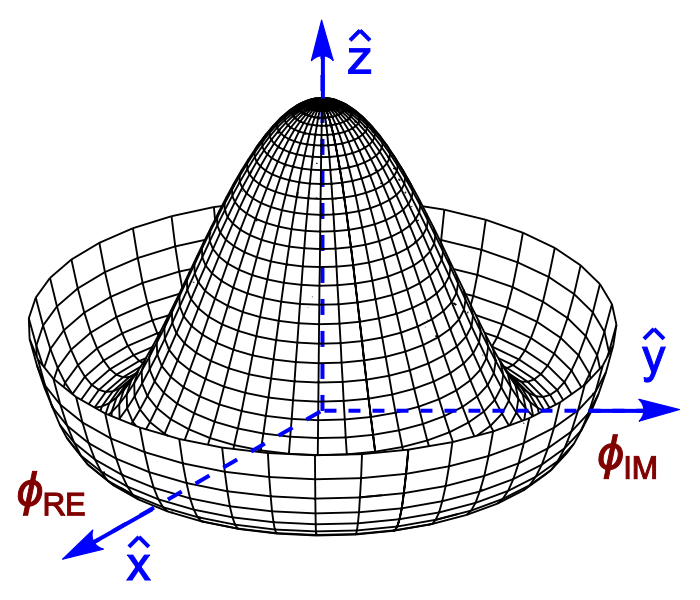
\includegraphics[width=0.6\textwidth]{figs/Mexican_hat.png}
    \caption{Complex scalar doublet potential.}
    \label{fig:MexicanHat}
  \end{center}
\end{figure}

\subsection{Brout-Englert-Higgs mechanism}
\label{sec:higgs}

After the spontaneous symmetry breaking, the scalar doublet transforms into the form given in equation~\ref{eq:TransHiggsDoublet}, where $G^{+}$ and $G^{0}$ are the Goldstone bosons from the breaking of the $SU(2)$ symmetry, and \Hb~is the Brout-Englert-Higgs boson. From Goldstone's theorem when a symmetry is spontaneously broken, a massless boson appears for each broken generator. In our specific case, the three generators of $SU(2)$ are broken giving rise to three Goldstone bosons: $G^{+}$, $G^{-}$ and $G^{0}$. This massless bosons are ``eaten'' by the $W^{+}$, $W^{-}$ and \Z~giving them an additional degree of freedom, the longitudinal polarization. 

\begin{equation}
  \label{eq:TransHiggsDoublet}
  \Phi=\left(
    \begin{array}{c}
      G^{+} \\
      \frac{1}{\sqrt(2)}(H+v-iG^{0})
    \end{array}
  \right)
\end{equation}

By this mechanism, the \W~and \Z~bosons acquire a mass, being its value set by the coupling constant of $SU(2)$ group and the vacuum expectation value of Brout-Englert-Higgs boson. In addition, the fermions in the theory also acquire a mass from the interactions with the scalar doublet. Such masses are in general of the form $m_{f}=\lambda_{f}v/\sqrt(2)$, where $\lambda_{f}$ sets the interaction between the Brout-Englert-Higgs boson and the fermion. Finally, also the Brout-Englert-Higgs boson has a mass $m_{H}^{2}=-2\mu^{2}$.

In summary, with this mechanism the weak interaction bosons and fermions of the theory are given a mass at the price of introducing at least one additional scalar field to spontaneously break the $SU(2)$ symmetry.

\section{Hierarchy problem and other SM limitations}
\label{sec:hier}

The SM is certainly one of the most successful theories in the history of physics. With only 19 free parameters, it is able to make thousands of predictions that have been measured and tested over the last seventy to eighty years. However some aspects in the model are not completely understood. The most important one is the so-called hierarchy mass problem. At tree level, the Brout-Englert-Higgs boson has a mass $m_{H}^{2}=-2\mu^{2}$, but the physical mass also contains the one-loop contributions from particles that interact with it, as the top quark. The Feynman diagram for such contribution can be seen in figure~\ref{fig:oneloophiggs}.

\begin{figure}[!Hhtbp]
  \begin{center}
    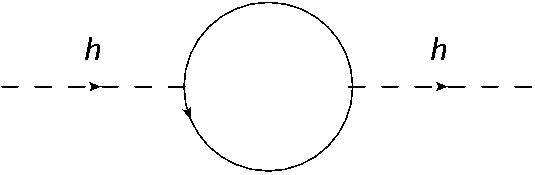
\includegraphics[width=0.6\textwidth]{figs/HierarchyLoop.png}
    \caption{One loop diagram for contributions to the mass of the Brout-Englert-Higgs boson from interactions with fermions.}
    \label{fig:oneloophiggs}
  \end{center}
\end{figure}

Such contributions add up giving a mass greater than simple tree level mass. Each fermion contributes proportionally to its mass, which means that the top quark contributes the most. Moreover, if there are in nature heavier fermions that also interact with the Brout-Englert-Higgs boson they will also contribute to its mass. With such considerations the Brout-Englert-Higgs boson mass is expected to be much greater than 125 GeV, and in principle not even of the order of 100 GeV but greater than 1 TeV. However the real relevance or significance of this problem at theoretical level has been discussed extensively, the majority of the community agrees there is something to be understood on the subject. 

The most famous proposed solution to this problem is supersymmetry (SUSY)~\cite{Fayet:1977yc,Martin:1997ns}. It proposes the existence of an additional symmetry between fermions and bosons, at a given point of the history of universe nature did not distinguish between fermions and bosons. However, as it is known, this does not happen presently, that means this symmetry must be broken. Such symmetry implies the existence of a super-symmetric partner for each particle, a super-partner. A fermion for each boson and vice versa. This SUSY procedure doubles the particle content of the model where it is applied. Before breaking SUSY, a particle and its partner have the same mass. This characteristic solves the hierarchy problem in SUSY. Figure~\ref{fig:susy} shows the one loop diagrams for the mass of the Brout-Englert-Higgs boson from the top and its super-partner the stop. Whereas, the top contribution is positive, the stop contribution is negative but equal in value, then cancelling each other.

\begin{figure}[!Hhtbp]
  \begin{center}
    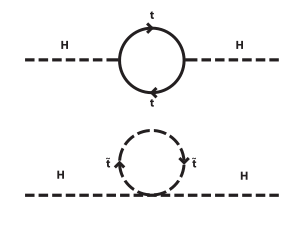
\includegraphics[width=0.6\textwidth]{figs/SUSY.png}
    \caption{One loop diagrams for contributions to the mass of the Brout-Englert-Higgs boson from the top and the stop.}
    \label{fig:susy}
  \end{center}
\end{figure}

But this solution works exactly only if SUSY is not broken. As SUSY has to be broken, different ways have been proposed to break SUSY and still offer a solution to the hierarchy problem, leading essentially to solutions that need a fine adjustment of the parameters of the theory. This represents for some theoreticians a problem itself: fine-tuning or naturalness. Extensive searches for SUSY particles have been performed, accordingly to different models: MSSM~\cite{Khachatryan:2014wca,Aad:2014vgg}, CMSSM~\cite{Agashe:2014kda}, etc.

While hierarchy problem is an internal problem of the SM, there are however several questions that have not been solved. For example, how gravity is understood in the frame of QFT's? Why there are only 3 generations of leptons and quarks? Why there are 4 fundamental forces? In addition, there have been experimental questionings to the SM. The most important one is the masses of neutrinos. In the SM neutrinos are massless, careful measurements~\cite{Ashie:2004mr, Weinheimer:2013hya} have shown that neutrinos can oscillate between different flavors, phenomenon only possible if neutrinos have a mass. Measurements of solar and atmospheric neutrino oscillations have been the most important proofs of physics beyond the SM. 

From cosmological measurements, the Wilkinson Microwave Anisotropy Probe (WMAP) has shown that the universe is not only made by visible matter, but suggests that around 24\% it is made of dark matter, a type of matter not visible by means of light. It has also shown that 71\% of the universe is composed of dark energy, which makes the universe to be in an accelerated state of expansion. These results are shown in~\cite{2013ApJS..208...20B, 2013ApJS..208...19H}. Also the Planck probe has shown similar results, for example in~\cite{Planck:2015xua}. The SM does not have any answer to these open problems so far. 

Finally, it is known that the universe presents an asymmetry between matter and antimatter, the first being much more abundant than the second. Such asymmetry can be obtained by CP-violating processes (C for charge and P for parity). However the amount of CP violation in the SM is not compatible with the huge matter-antimatter asymmetry in nature. This problem, known as baryon asymmetry, represents an additional huge challenge for particle physics. 

In conclusion, the SM has been a formidable model that has helped the understanding of a huge amount of physics. It has done thousands of predictions that have been verified experimentally in the last half-century. However, this is not the end of the story, perhaps only the beginning. There are theoretical and experimental motivations that support the idea that the SM is not the ``final'' theory that could explain all subatomic phenomena in nature. Currently, there are a lot of efforts, both theoretical and experimental, to understand and explain all the remaining pieces. The present work is one of them.

In the next section, an extension of the SM that looks for a solution to the discussed hierarchy problem is presented. Chapter~\ref{chap:pheno} shows a strategy to look at LHC data for some of the predictions given by this SM extension.  %Then, principal productions predicted by the SM at the LHC involving particles, the top and the Higgs, used for new physics searches will be described. 

\section{Vector Like Quarks}

\label{chap:VLQ}

From last sections it has been shown how there are some parts in the SM that need further understanding. From such internal issues some further models/theories have been developed. All this theories are commonly grouped under the term Beyond Standard Model or simply BSM. As already mentioned, one of the most famous BSM theory is supersymmetry (SUSY). This idea have given birth to a plethora of model realizations and physics predictions. So far, none of the new consequences of this theory have been confirmed but the experiments have an enormous investment on their search. But not only SUSY have seen the day light, there is on the market an astonishing amount of BSM theories addressing different issues of the SM. Extra dimensions, fourth families, composite Higgs are a few of them.

In this section a bunch of models that introduce additional heavy quarks, heavier than the top, in order to solve the hierarchy problem will be described. %, described in section~\ref{sec:hier}. 

\subsection{Theoretical motivation}
\label{sec:motiv}

Even though the SM has 3 families, the number of families in nature is not restricted by any fundamental principle. However, searches for fourth families have not found any evidence of additional families in nature~\cite{Eberhardt:2012gv}. But a fourth family formulation relies on the existence of a sequential additional family, this is for the quark sector, two additional quarks, heavier than the top with the same quantum number structure as the other 3 families. In particular the 3 SM families are formed by doublets of the left components of quark fields. 

Fermionic fields can be divided in terms of two chiral components. The chirality is related to the relative orientation of the momentum and spin of a particle. A particle is said to have right chirality if its momentum and spin are aligned and left chirality if they are anti-aligned.  Accordingly to electroweak theory the only left fermions undergo weak interactions, reason why SM quark families are left. 

Nothing prevents to formulate a model where new quarks right and left components are subjected to weak interaction indistinctly. A fermion having identical left and right chiralities is called vector-like. These type of models introduce only new quarks without the need of a full new family.

This new top-like states allow to have a suitable solution for the hierarchy problem. They arise typically in Kaluza-Klein extra dimension models~\cite{Kaluza:1921tu, Contino:2006qr, Matsedonskyi:2012ym, Dissertori:2010ug}. In more generic modeling of vector-like quarks (VLQ)~\cite{Aguilar-Saavedra:2013qpa, Buchkremer:2013bha} these new states are added to the SM content as an electroweak representation (singlet or doublet) coupled to SM quarks.

\subsection{Generic Formulation}
\label{sec:form}

The generic formulation that is going to be described is based on~\cite{Buchkremer:2013bha, Cacciapaglia:2011fx}.

In a very generic conception, vector-like quarks can be added to the SM content as being part of an electroweak representation. Introduced with the same color charge than SM quarks they can come in 4 different forms depending of their electric charge:
\begin{itemize}
\item $X$ with 5/3 electric charge
\item \Tp~with 2/3 electric charge, as the top quark.
\item $B$ with -1/3 electric charge, as the bottom quark.
\item $Y$ with -4/3 electric charge.
\end{itemize}

The \Tp~is also called in the literature a top partner. Given the VLQ electric charges, they can be arranged in different representations. Table~\ref{tab:VLQRepre} displays the plausible different electroweak representations of VLQ. The $\binom{X}{T}$ and $\binom{T}{B}$ doublet will referred as the non-standard and standard doublet respectively.  

\begin{table}[htbH]
\begin{center}
\begin{tabular}{|c|c|c|c|c|c|c|}
\hline 
 & SM & \multicolumn{2}{c|}{Singlets} & \multicolumn{3}{c|}{Doublets} \\
 & $\binom{u}{d}$ $\binom{c}{s}$ $\binom{b}{t}$ & \Tp & B & $\binom{X}{T'}$ & $\binom{T'}{B}$ & $\binom{B}{Y}$ \\ 
\hline
$SU(2)_{L}$ & 2 & \multicolumn{2}{c|}{1} & \multicolumn{3}{c|}{2} \\ \hline
$U(1)_{Y}$ & $q_{L}=1/6$; $u_{R}=2/3$; $d_{R}=-1/3$ & 2/3 & -1/3 & 1/6 & 7/6 & -5/6 \\
\hline
\end{tabular}
\caption{Possible VLQ representations and corresponding $SU(2)_{L}\times U(1)$ charges and SM quarks. \label{tab:VLQRepre}}
\end{center}
\end{table}

The effective Lagrangian for a general formulation of VLQ, restricting it for \Tp~and $X$ type of vector-like quarks in the non-standard doublet is the following:
\begin{eqnarray}
  \mathcal{L} & = & \kappa_{T}\left\{ \sqrt{\frac{\zeta_{i}\xi_{Z}^{T}}{\Gamma_{Z}^{0}}}\frac{g}{2c_{W}}\left[ \bar{T'}_{R}Z_{\mu}\gamma^{\mu}u^{i}_{R}\right]\right\} 
               -  \kappa_{T}\left\{ \sqrt{\frac{\zeta_{i}\xi_{H}^{T}}{\Gamma_{H}^{0}}}\frac{M}{v}\left[ \bar{T'}_{L}Hu^{i}_{R}\right] + \sqrt{\frac{\zeta_{3}\xi_{H}^{T}}{\Gamma_{H}^{0}}}\frac{m_{t}}{v}\left[ \bar{T'}_{R}Ht_{L}\right]\right\} \nonumber\\            
              & + & \kappa_{X}\left\{ \sqrt{\frac{\zeta_{i}}{\Gamma_{W}^{0}}}\frac{g}{\sqrt{2}}\left[ \bar{X}_{R}W^{+}_{\mu}\gamma^{\mu}u^{i}_{R}\right]\right\} +h.c.
\label{eq:VLQLag}
\end{eqnarray} 
neglecting terms proportional to the light quark masses. In addition, terms proportional to top mass can also be neglected as they only introduce differences of only 10\%-20\% for \Tp~masses below 600 GeV. The parameters $\kappa_T$, $\kappa_X$ are the coupling strengths and determine the strength of the VLQ production. In equation~\ref{eq:VLQLag}, $M$ represents the \Tp~mass, $m_{t}$ the top mass, $\zeta_{i}$ the coupling between VLQ and the $i$th SM quarks generation, $\xi_{Z}^{T}$ and $\xi_{H}^{T}$  the mixing of \Tp~with the $Z$ and Higgs boson respectively. Finally, $v$ and $g$ are the usual vacuum expectation value and electroweak coupling in the SM, and $\Gamma^{0}_{i}$ the width of the boson $i=W^{+/-},Z^{0},H^{0}$.
%\begin{TOINCLUDE}Table with different possible representations and assigned charges\end{TOINCLUDE}

\subsubsection{Production modes}
\label{sec:prod}

VLQ can be produced singly or pairwise, as the SM top quark. Pair production is dominated by QCD processes via gluons, as shown in figure~\ref{fig:ProdDiagPair}. Additional contributions are given via the t-channel exchange of a vector boson. For example, figure~\ref{fig:ProdDiagPair} shows the production process via the \Z~boson that produce two same sign VLQ.   

Single production is mainly mediated by a vector boson via a t-channel in association with a SM quark. In figure~\ref{fig:ProdDiagSingle} the Feynman diagram for \Tp~single production with a SM quark is shown. In addition, the \Tp~can be also produced with a \Z~or \W~boson or a Higgs from an initial gluon-quark fusion. 

The VLQ production cross section in proton-proton collision strongly depends of their mixings to SM quarks. Historically, top partners have been modeled with exclusive mixings to third generation SM quarks. In the generic formulation being considered, the VLQ can mix to the three SM quark generations. In particular the case where couplings to light generations are important has been considered for the present work. Figure~\ref{fig:TProdXS},~\cite{Cacciapaglia:2011fx}, shows the \Tp~production cross sections in pairs and singly in proton-proton collisions. For \Tp~masses higher than 500~\GeVcc the single production is dominant with regard to pair production, at 8~TeV center of mass energy . 

\begin{figure}[!Hhtbp]
  \begin{center}
    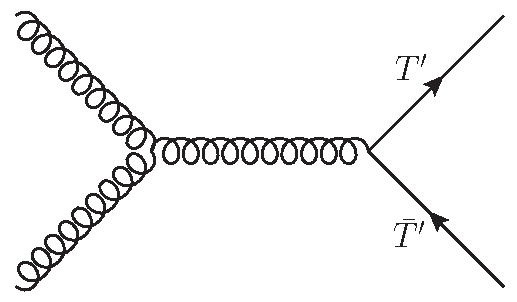
\includegraphics[width=0.3\textwidth]{figs/Gluon_fusion_T_pair.jpg}
    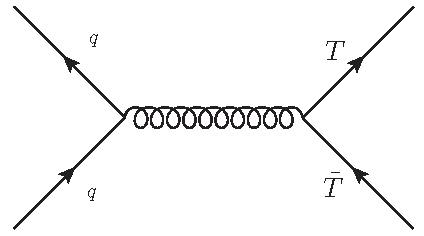
\includegraphics[width=0.3\textwidth]{figs/Quarks_schannel_T_pair.jpg}
    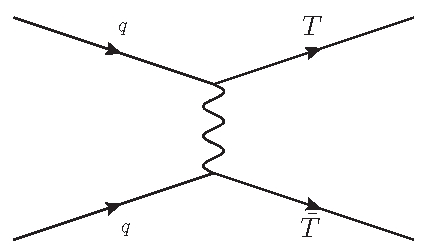
\includegraphics[width=0.3\textwidth]{figs/Gluon_tchannel_T_pair.jpg}
    \caption{Feynman diagrams of \Tp~production in pairs.}
    \label{fig:ProdDiagPair}
  \end{center}
\end{figure}

\begin{figure}[!Hhtbp]
  \begin{center}
    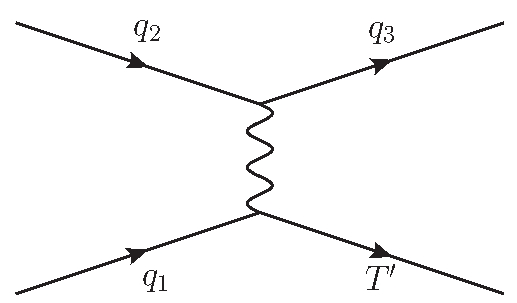
\includegraphics[width=0.45\textwidth]{figs/Tchannel_T_single.jpg}
    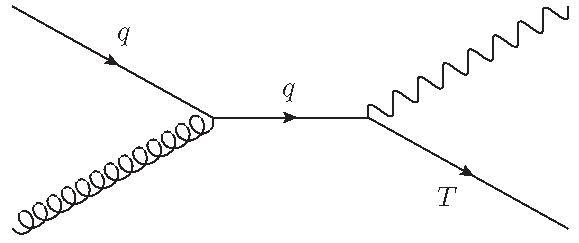
\includegraphics[width=0.45\textwidth]{figs/QuarkGluonFusion_SingleT.jpg}
    \caption{Single \Tp~production Feynman diagrams.}
    \label{fig:ProdDiagSingle}
  \end{center}
\end{figure}

\begin{figure}[!Hhtbp]
  \begin{center}
    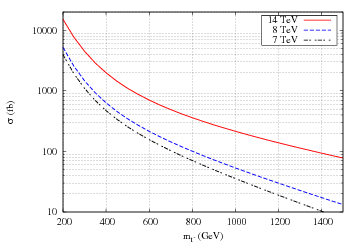
\includegraphics[width=0.45\textwidth]{figs/pheno_prod_single_tp.png}
    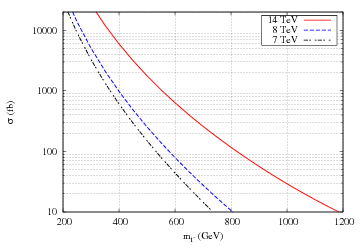
\includegraphics[width=0.45\textwidth]{figs/pheno_prod_pair_tp.png}
    \caption{\Tp~production cross section for single [left] and pair [right] channels as a function of \Tp~mass for different center of mass energy in proton-proton collisions~\cite{Cacciapaglia:2011fx}.}
    \label{fig:TProdXS}
  \end{center}
\end{figure}
%\begin{TOINCLUDE}Plot of production cross section at LHC for different energies as a function of the mass. Feynman diagrams of the production processes.\end{TOINCLUDE}

\subsubsection{Decay modes}
\label{sec:decay}

The parameters $\zeta_{i}$ and $\xi_i$, from the Lagrangian in equation~\ref{eq:VLQLag}, are directly linked to the branching ratios:
 \begin{eqnarray} 
BR (T' \to Z^{0} j) = \frac{\zeta_{jet} \xi^T_Z}{1+\zeta_3 \xi_H \delta_H}\,, & & BR (T' \to Z^{0} t) = \frac{(1-\zeta_{jet}) \xi^T_Z}{1+\zeta_3 
\xi_H \delta_H}\,,\\
BR(T' \to H^{0} j) = \frac{\zeta_{jet} (1-\xi^T_Z)}{1+\zeta_3 \xi_H \delta_H}\,, & &  BR(T' \to H^{0} t) = \frac{(1-\zeta_{jet})
(1-\xi^T_Z) (1+\delta_H)}{1+\zeta_3 \xi_H \delta_H}\,, \nonumber\\
 & & \nonumber \\
BR(X \to W^{+} j) = \zeta_{jet}\,, & & BR(X \to W^{+} t) = (1-\zeta_{jet})
 \end{eqnarray} where $\zeta_{jet}$ accounts for the contributions of the two light quark generations and $j$ for jet.

The branching fractions of the top partner \Tp~only depend on the two parameters $\zeta_{jet}$ and $\xi_Z^{T}$, as $\delta_H$ is a calculable function of the heavy mass scale for the vector-like quarks $M$:
\begin{eqnarray} 
\delta_H  \sim 5 \frac{m^2_t}{M^2}\,, \label{eq:deltaH}
\end{eqnarray} 
where only the leading order in $1/M^2$ has been kept. Note that in these formulae the decay rates into \Z~and \Hb~are kept arbitrary (parameterised by $\xi_Z^{T}$ which is equal to 1/2 for the non-standard doublet case). These approximate but quite robust results allow to describe easily the phenomenology of the non-standard doublet. 

For a \Tp~coming from other representations the situation is not much different in terms of decay modes, as only the extra decay to \W~boson and quarks will be present. In figure~\ref{fig:TBRs} are presented the branching ratios of \Tp~as a function of its mass~\cite{Cacciapaglia:2011fx}. It is important to notice that for masses higher than 300~\GeVcc~the decay channel into top-Higgs becomes dominant.

\begin{figure}[!Hhtbp]
  \begin{center}
    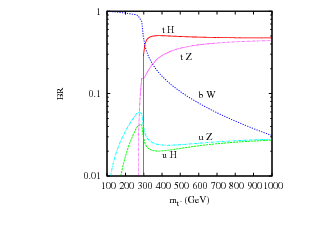
\includegraphics[width=0.8\textwidth]{figs/pheno_br_tp.png}
    \caption{\Tp~branching ratios as a function of its mass~\cite{Cacciapaglia:2011fx}.}
    \label{fig:TBRs}
  \end{center}
\end{figure}

In the present work, a search for a \Tp~will be described. This search looked for the \Tp~when it decays into a top quark and a Higgs boson. Therefore is important to understand the properties of these particles and how they are produced in the LHC, as predicted by the SM. In the next sections the production of these SM particles at the LHC and their specific properties are going to be presented. %In particular the top and the Higgs, constantly used for new physics searches will be described.

\section{Top at the LHC}
\subsection{Top production}

Discovered in 1995,~\cite{Abe:1995hr, Abachi:1995iq}, by D\O~\cite{Abazov:2002su} and CDF~\cite{Blair:1996kx} collaborations at Tevatron~\cite{Group:1984bk}, it is the heaviest known fundamental particle. As heaviest particle, many models beyond the SM predict a coupling of the top quarks with a heavier new physics sector. It forms a $SU(2)_{L}$ weak isospin doublet with the b-quark, discovered in 1977~\cite{Herb:1977ek}. Their mass difference, two orders of magnitude, is a fundamental question in the SM. Precision measurements of the top quark characteristics are fundamental inputs to test the SM and new physics searches.

The LHC can be seen as a top-factory, being the accelerator where the most of top-quarks can be produced. The top quark is produced in pairs and single production mode. During run 1, taking into account 7 TeV and 8 TeV data, 5.6 millions of top pairs events and 2.7 millions of single top events were delivered by the LHC to ATLAS and CMS experiments. Taking into account the different cross sections of the production processes, that will be discussed in the following sections, and the instantaneous luminosity, cited in table~\ref{tab:LHCparams}, for 8 TeV center of mass energy, at LHC around 6 tops per second are produced, where 5 of them come from top-pair events and one from single-top events.  

\subsubsection{Pair production}
\label{subsec:toppair}

Top pair production constitutes the dominant production channel in proton-proton collisions at LHC. Its high cross section makes this process one of the most important background for searches of new physics at LHC. Latest theoretical calculations at Next-to-Next-to-Leading-Order (NNLO)~\cite{Czakon:2013goa}, see section~\ref{sec:parton}, of top pair production from proton-proton collisions at $\sqrt{s}=8$ TeV give a cross section $\sigma_{t\bar{t}}=247.47$ pb with around 5\% total uncertainty. The tree level diagrams that contribute to this production are summarized in figure~\ref{fig:PairProductionFD}, where gluon fusion dominates the pair production. At $\sqrt{s}=13$ TeV, as for LHC Run 2, this cross section will scale about 3.3 times. Comparison between theoretical predictions and experimental measurements of top pair production is shown in figure~\ref{fig:PairProduction}~\cite{TOPLHCWG}.

\begin{figure}[!Hhtbp]
  \begin{center}
    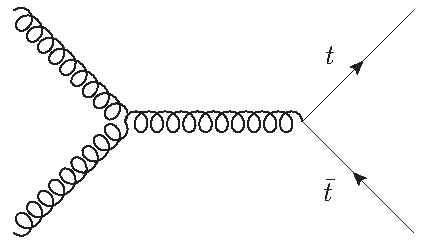
\includegraphics[width=0.32\textwidth]{figs/Gluon_fusion_top_pair.jpg}
    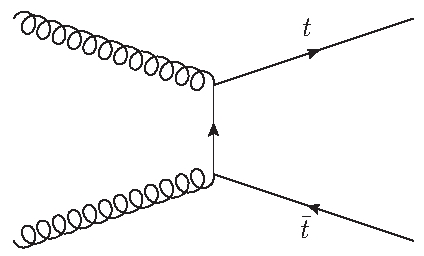
\includegraphics[width=0.32\textwidth]{figs/Gluon_tchannel_top_pair.jpg}
    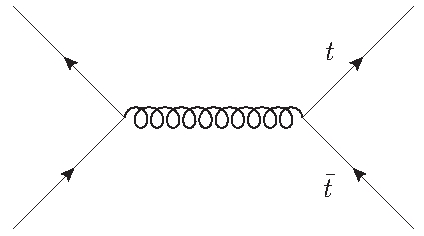
\includegraphics[width=0.32\textwidth]{figs/Quarks_schannel_top_pair.jpg}
    \caption{Top pair production processes Feynman diagrams for proton-proton collisions, via gluon fusion [left], gluon t-channel [middle] and quark-antiquark annihilation [right].}
    \label{fig:PairProductionFD}
  \end{center}
\end{figure}

\begin{figure}[!Hhtbp]
  \begin{center}
    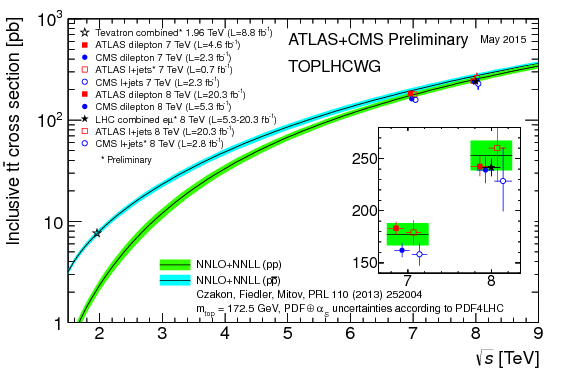
\includegraphics[width=0.9\textwidth]{figs/toplhcwg_ttxsec_sqrts_may2015.png}
    \caption{$t\bar{t}$ production cross section as a function of the center of mass energy in $p\bar{p}$ and $pp$ collisions compared to theoretical predictions~\cite{TOPLHCWG}.}
    \label{fig:PairProduction}
  \end{center}
\end{figure}

%\begin{TOINCLUDE}Plots of cross section of ttbar production as a function of center of mass energy; Feynman diagrams for pair production\end{TOINCLUDE}

\subsubsection{Single $t$ production}
\label{subsec:topsing}

A subdominant production process of top quark is the single production channel, where the top quark is produced in association with another quark, mediated by a $W$ boson, or with a $W$ boson. The Feynman diagrams for tree level single top production can be seen in figure~\ref{fig:SingleProductionFD}. NNLO predictions have been also done for these three single production modes, at $\sqrt{s}=8$ TeV. The cross sections are respectively: $\sigma_{t,\; \text{s-channel}}=5.56\pm0.22$ pb, $\sigma_{t,\; \text{t-channel}}=84.34\pm1.69$ pb and $\sigma_{tW}=22.2\pm0.67$ pb. Due to the high cross section of pair production compared to single production channels, the cross section measurement of each production mode has been difficult. The Tevatron was able to confirm the $s$ and $t$-channels~\cite{Abazov:2009ii, Aaltonen:2009jj}, while at LHC the $tW$ channel was confirmed~\cite{Aad:2012xca, Chatrchyan:1642680}. The comparison of theoretical predicted cross section and experimental measurements, by ATLAS and CMS, at different center of mass energies is p[resented in figure~\ref{fig:SingleProduction}~\cite{TOPLHCWG}.

\begin{figure}[!Hhtbp]
  \begin{center}
    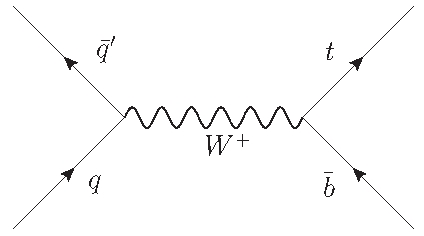
\includegraphics[width=0.32\textwidth]{figs/Schannel_top_single.jpg}
    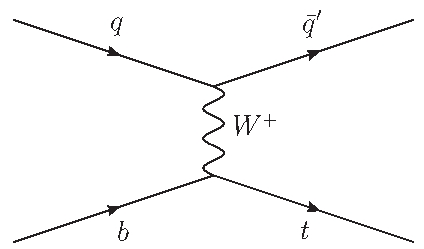
\includegraphics[width=0.32\textwidth]{figs/Tchannel_top_single.jpg}
    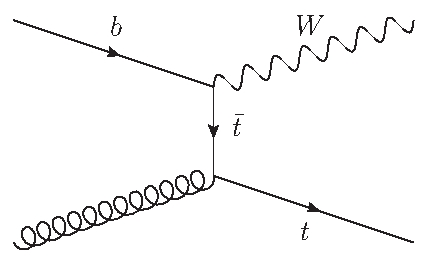
\includegraphics[width=0.32\textwidth]{figs/TWchannel_top_single.jpg}
    \caption{Feynman diagrams of single top production processes of proton-proton collisions, from left to right s-channel, t-channel and associated \W~production.}
    \label{fig:SingleProductionFD}
  \end{center}
\end{figure}

\begin{figure}[!Hhtbp]
  \begin{center}
    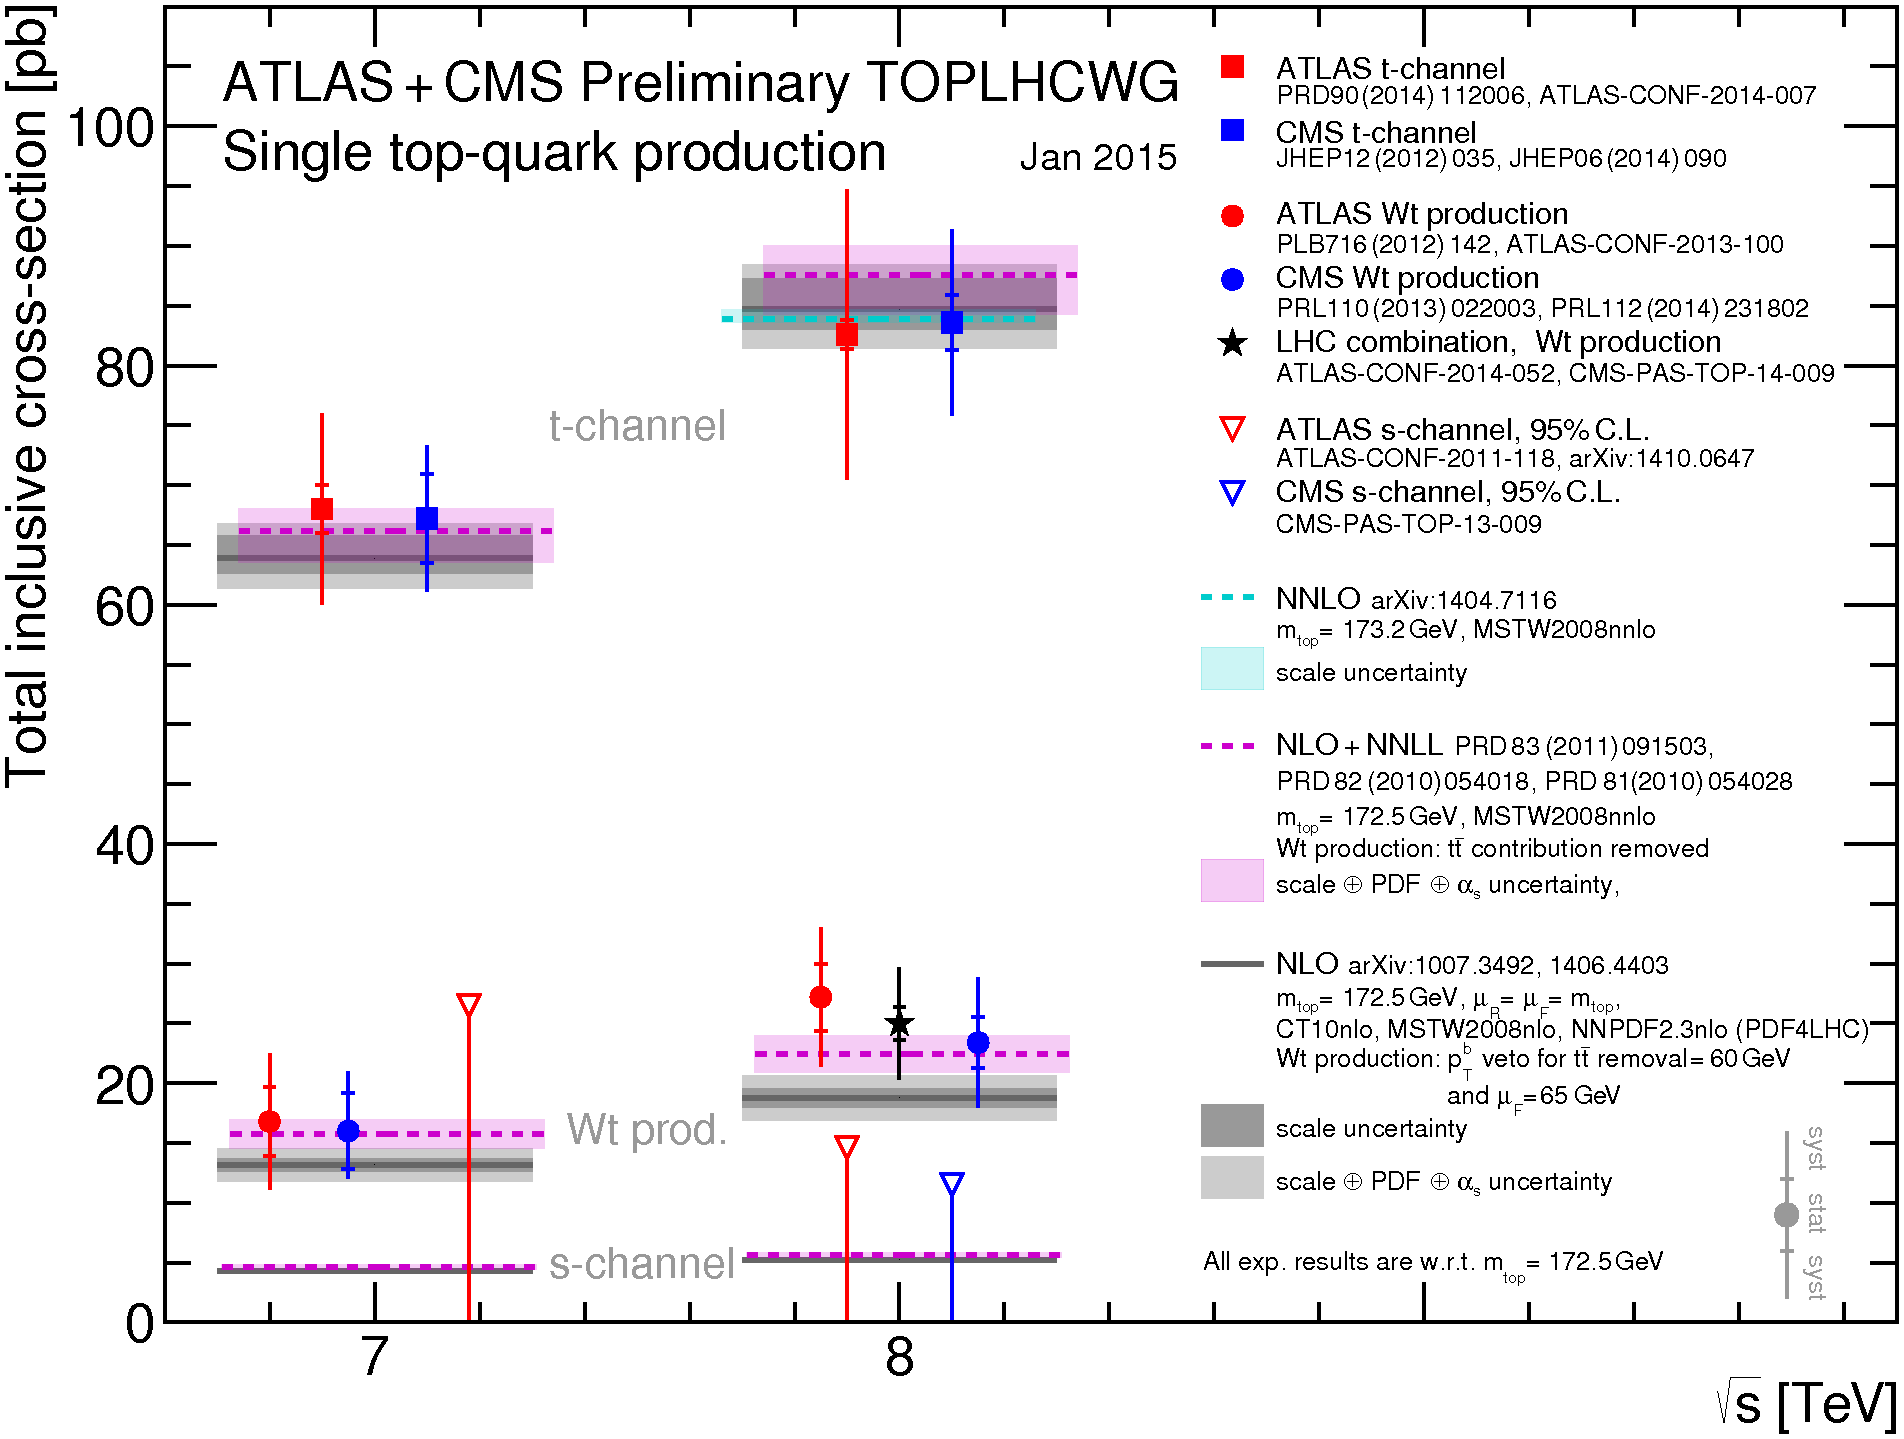
\includegraphics[width=0.9\textwidth]{figs/singletop_allchanvsroots.png}
    \caption{Single top production cross section as a function of the center of mass energy in proton-proton collisions compared to theoretical predictions for each production channel by ATLAS and CMS collaborations~\cite{TOPLHCWG}.}
    \label{fig:SingleProduction}
  \end{center}
\end{figure}

%\begin{TOINCLUDE}Plots of cross section of single-top production as a function of center of mass energy; Feynman diagrams for single production\end{TOINCLUDE}

\subsection{Top decay channels}

The top quark decays extremely fast, a process taking only $3\times 10^{-25}$ second. Hadronization processes occur around $3\times 10^{-24}$ which means that the top quark decays even before hadronization begins. Therefore it is the only quark that can be studied before hadronization, in its free state. \\ According to CKM matrix (Cabibbo–Kobayashi–Maskawa)~\cite{PhysRevLett.10.531, Kobayashi01021973}, that describes how different quarks interact between them, the top quark decays preferentially to a b-quark and a $W$ boson, 99\% of the times~\cite{Agashe:2014kda}. 

Then \W boson can decay into a lepton and a neutrino, or into a pair of quarks. The branching ratio of leptonic decays of \W boson is around 33\% while to quarks is 67\%~\cite{Agashe:2014kda}, being dominant then the hadronic final state. In figure~\ref{fig:BRratiosandDecayChannels} can be seen the two decay modes of top quark with their respective branching ratio. 

\begin{figure}[!Hhtbp]
  \begin{center}
    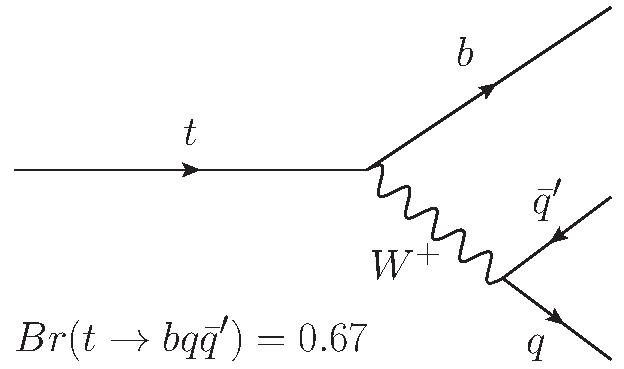
\includegraphics[width=0.4\textwidth]{figs/Top_H_Decay.png}
    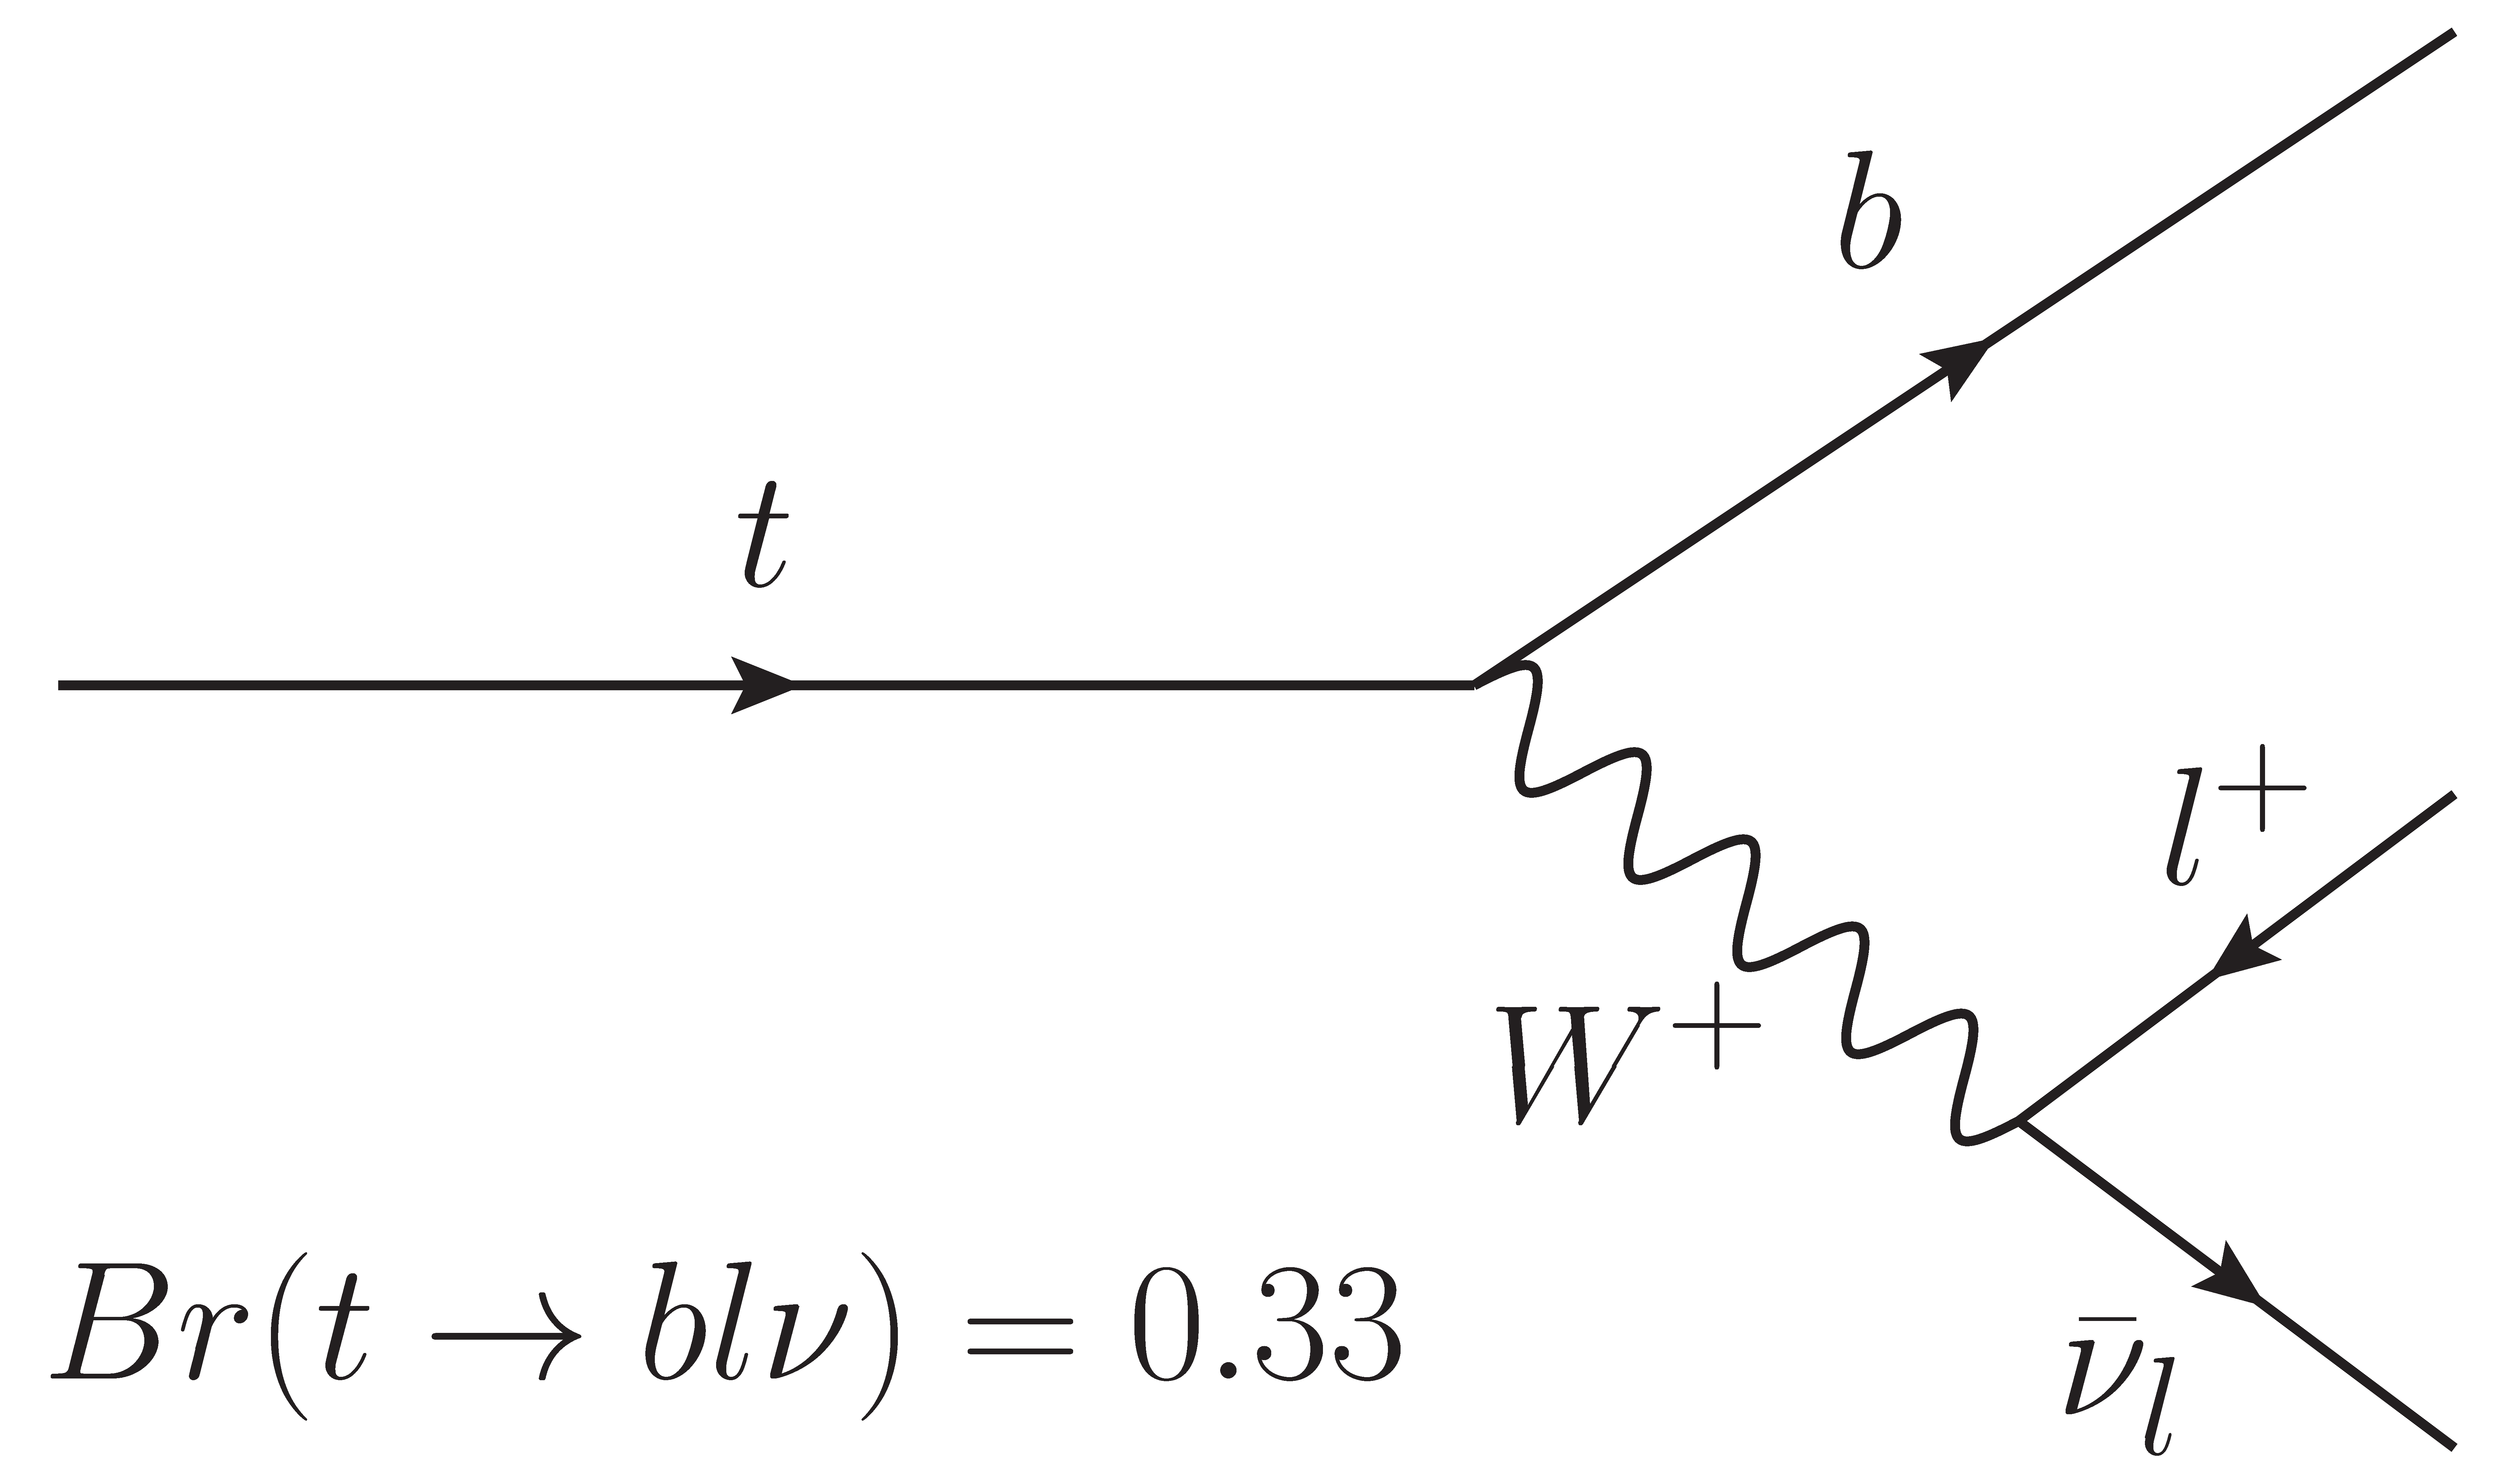
\includegraphics[width=0.4\textwidth]{figs/Top_L_Decay.png}
    \caption{Feynman diagrams for top decay channels with respective branching ratios.}
    \label{fig:BRratiosandDecayChannels}
  \end{center}
\end{figure}

%\begin{TOINCLUDE}Plot on possible decay channels and branching ratios to each channel; Feynman diagram for each decay channel\end{TOINCLUDE}
%
%\subsection{Top properties}
%
%Description of top properties and the measurement of them.
%
%\subsubsection{Electric charge}
%
%Top charge related to its decay.
%
%\subsubsection{Lifetime}
%
%Discussion on the importance of measurements of top as only quark decaying before hadronization time.

\subsection{Mass and width of top quark}

One of the most important quests in top physics is the measurement of top mass and width. They constitute two powerful tests of SM predictions. Whereas the top mass is a free parameter in the SM, it is constrained by other measurements, specially electroweak precision tests. Any deviation with respect to the expectation of the SM could point to the existence of new physics beyond the standard model. The width is also predicted by the SM.% and then it needs to be measured in experiment. 

At Next-to-Leading-Order (NLO)~\cite{Jezabek19891}, the SM expected value of top width is $\Gamma_{t}=1.27$ GeV. It depends of the top mass, the strong force coupling $\alpha_{S}$, the mass of the \W~boson and the strength of the interaction between the top and b-quark. Present measurements have found $\Gamma_{t}=2.00^{+0.47}_{-0.43}$ GeV~\cite{Abazov:2012vd}, value in agreement with SM predictions. 

Top mass has been measured by ATLAS and CMS collaborations at LHC and by CDF and D\O~at Tevatron for each decay channel of top both in single and pair production. Current world combination is $m_{t}=173.34\pm 0.76$. Results from current searches and their combinations are presented in figure~\ref{fig:TopMass}~\cite{TOPLHCWG}. 

\begin{figure}[!Hhtbp]
  \begin{center}
    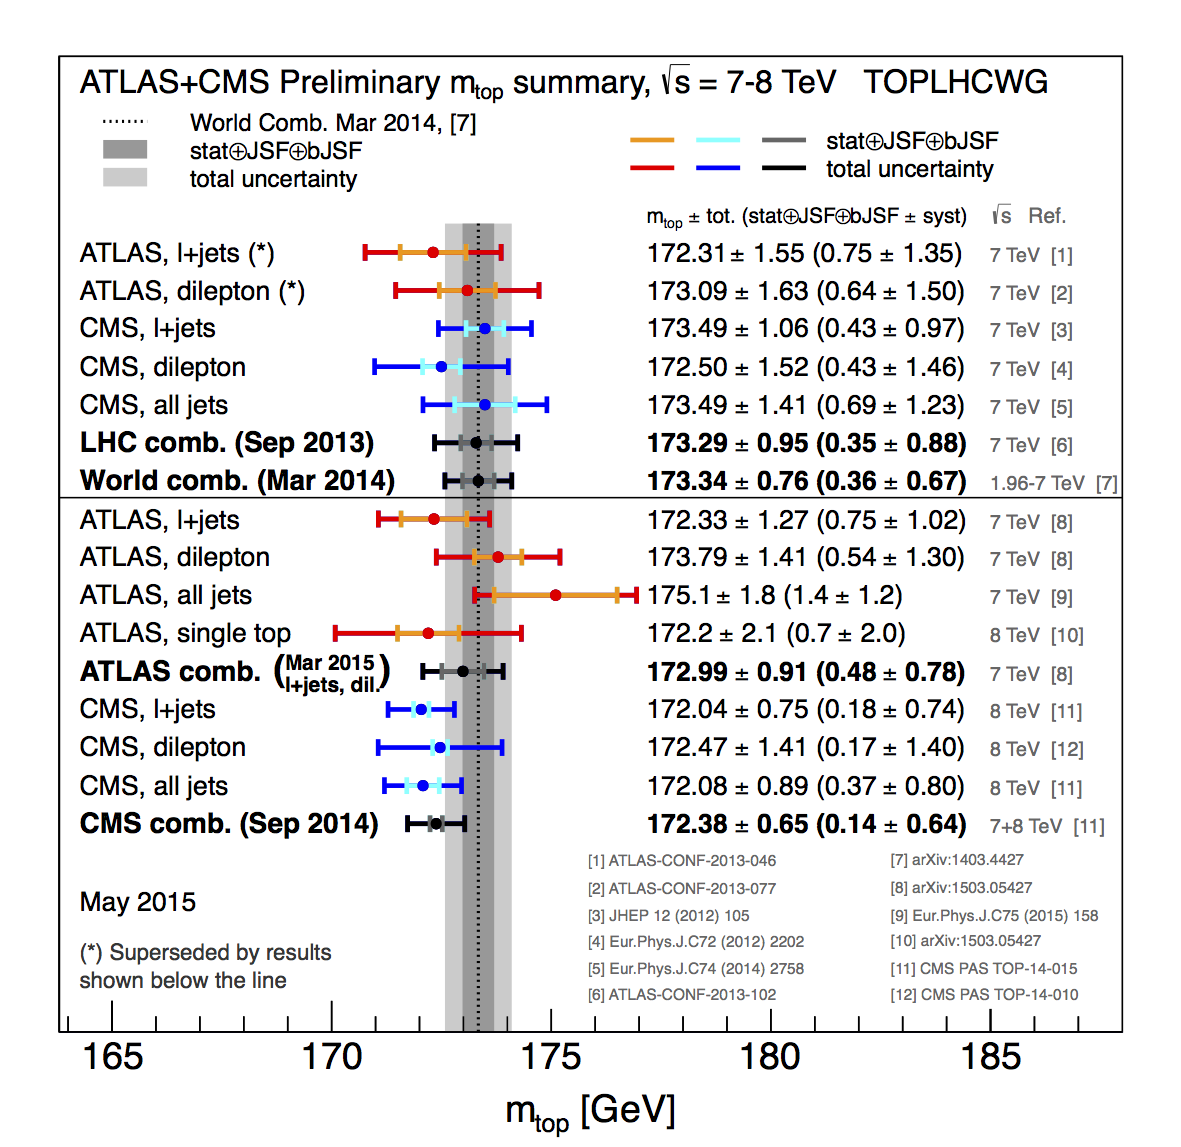
\includegraphics[width=0.9\textwidth]{figs/LHC_topmass_May2015.png}
    \caption{Top mass measurements from ATLAS and CMS collaborations and world combination including Tevatron results~\cite{TOPLHCWG}.}
    \label{fig:TopMass}
  \end{center}
\end{figure}

%\begin{TOINCLUDE}Plot of top mass measurement from Tevatron+LHC combination\end{TOINCLUDE}
%
%\subsubsection{Spin correlation}
%
%Discussion on how ttbar system have spin correlation that will be important for precision measurements.

\section{Higgs at the LHC}
\subsection{Higgs production}

The SM Higgs boson is expected to be produced in proton-proton collisions at LHC by four different processes: gluon fusion, via the fusion of two gluons via a top loop, Higgsstrahlung, where a Higgs boson is radiated from a \Z~or \W~boson, vector boson fusion, by the fusion of two vector bosons radiated from quarks, and quark fusion, from the fusion of quarks produced by a gluon splitting. Feynman diagrams for these processes are shown in figure~\ref{fig:HiggsProd}. 

\begin{figure}[!Hhtbp]
  \begin{center}
    \includegraphics[width=0.42\textwidth, height=4cm]{figs/GluonFusion_H.png}
    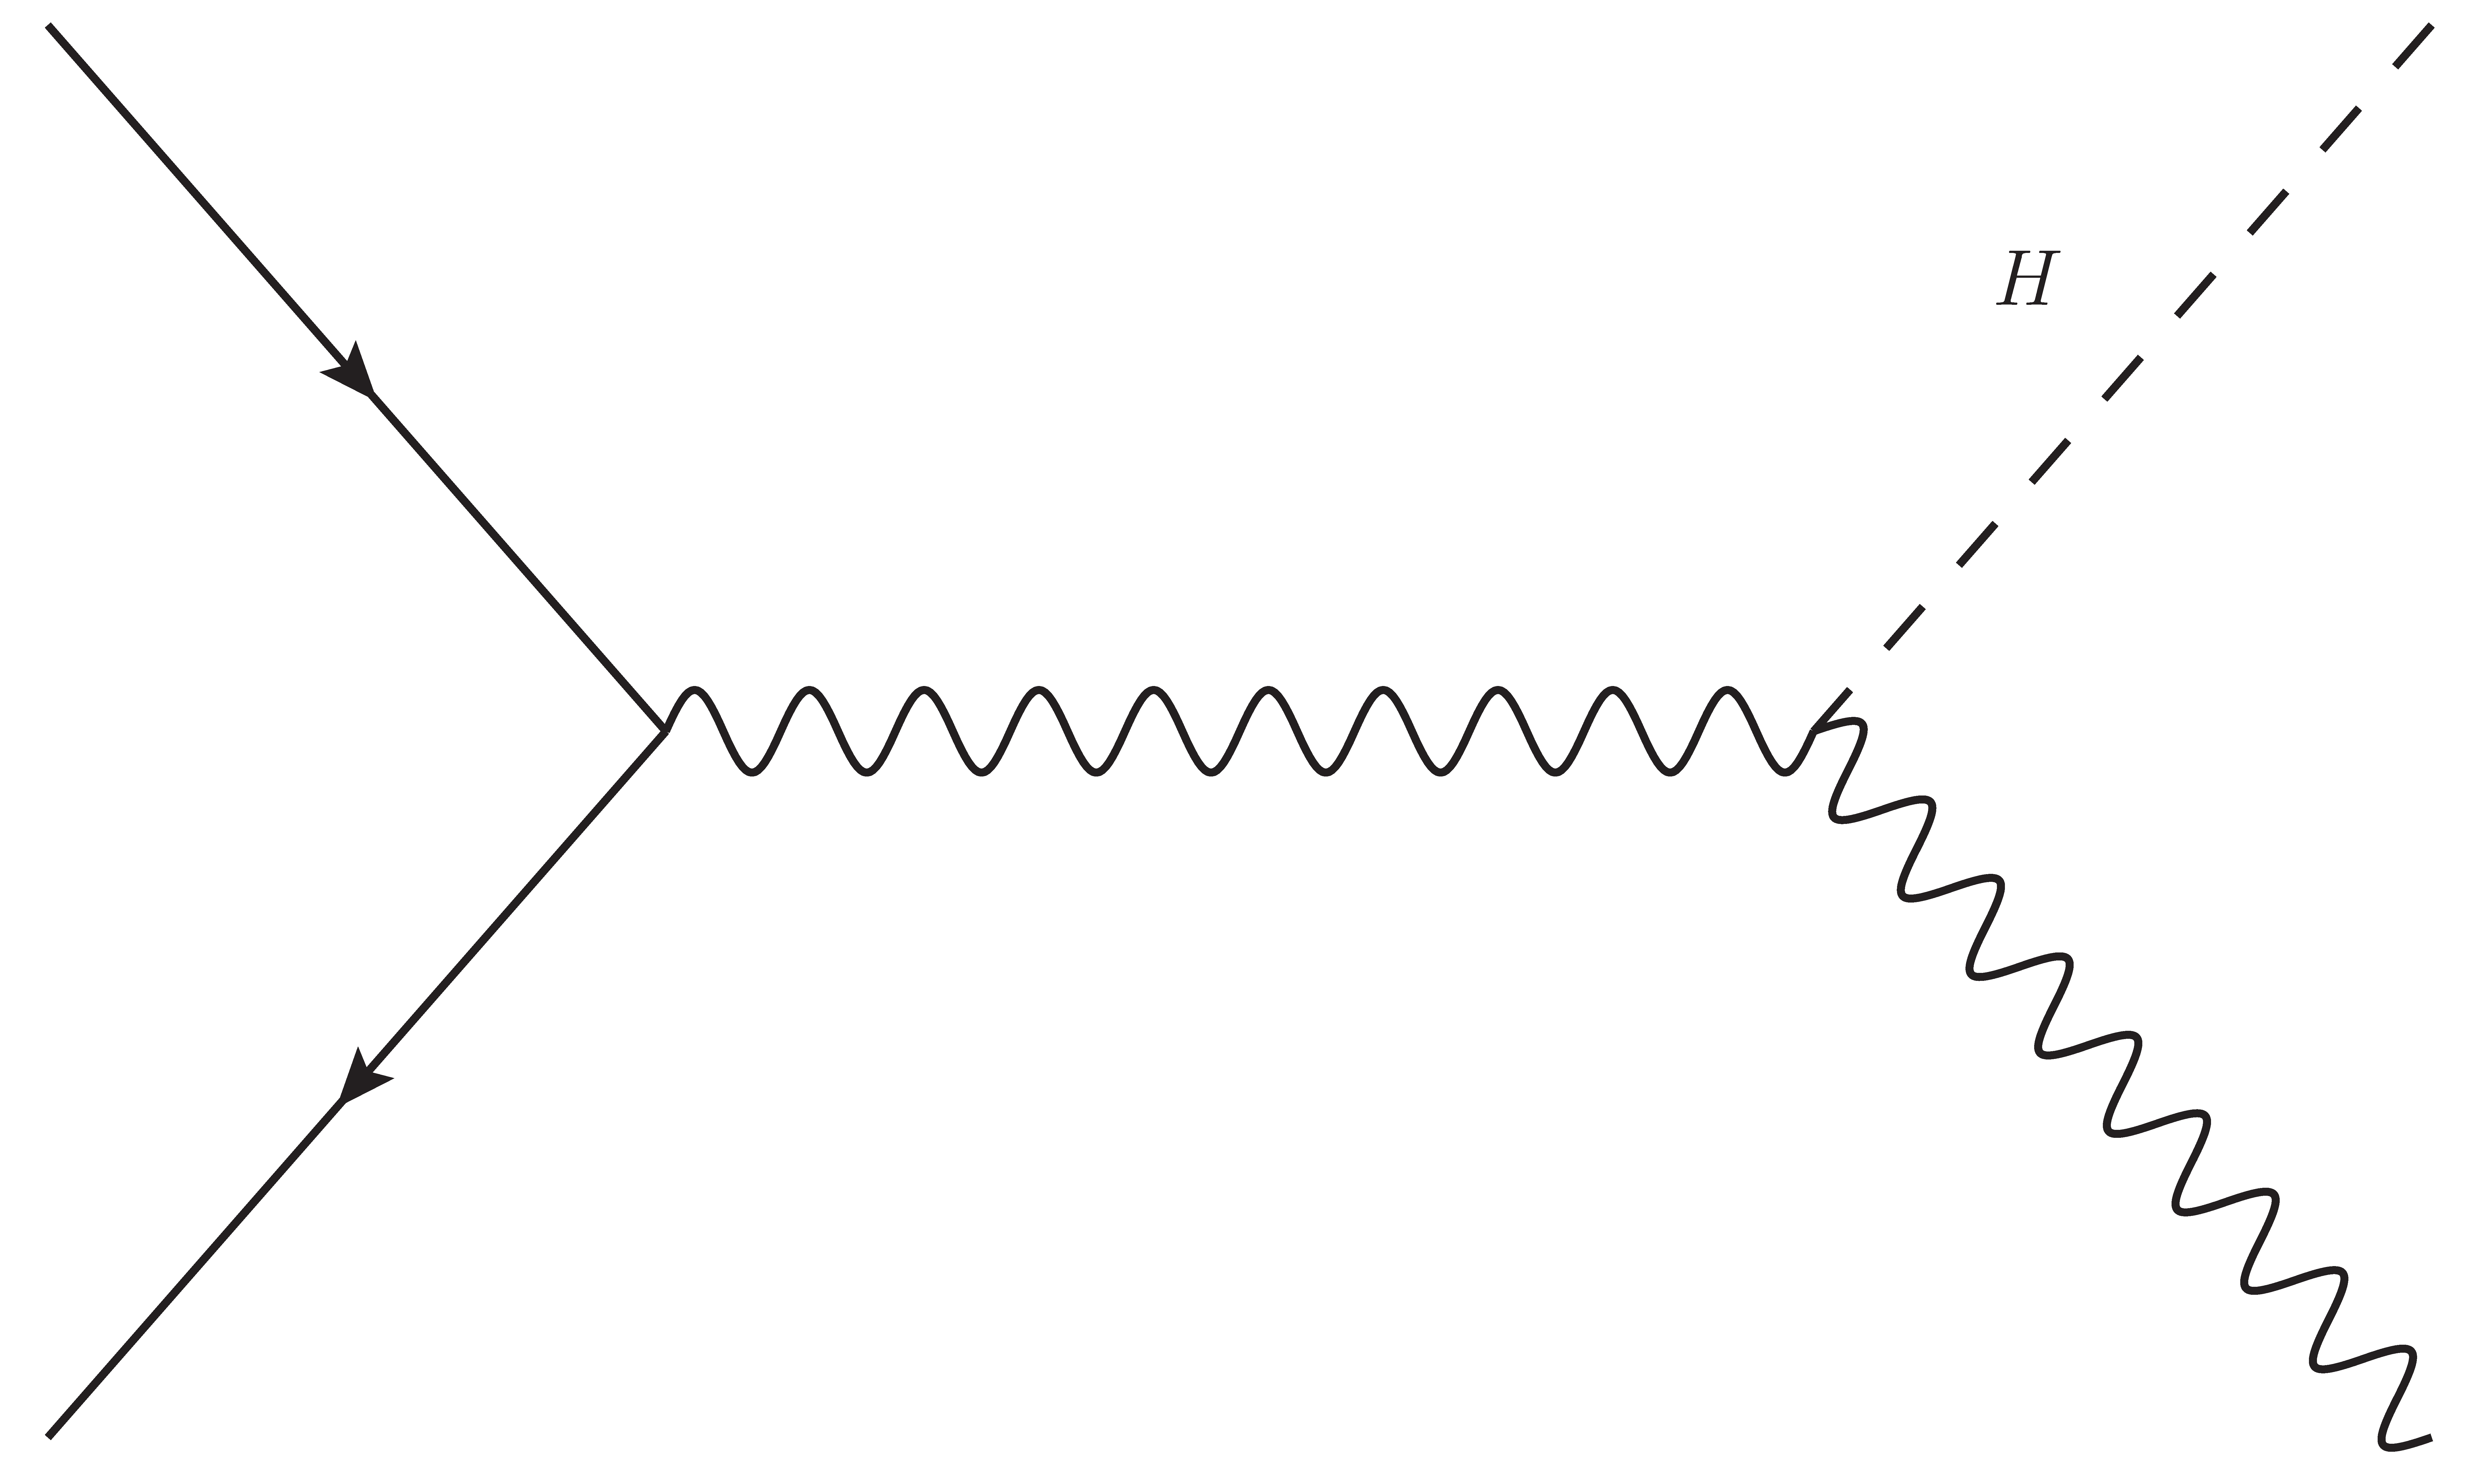
\includegraphics[width=0.42\textwidth, height=4cm]{figs/Higgstrahlung.png}
    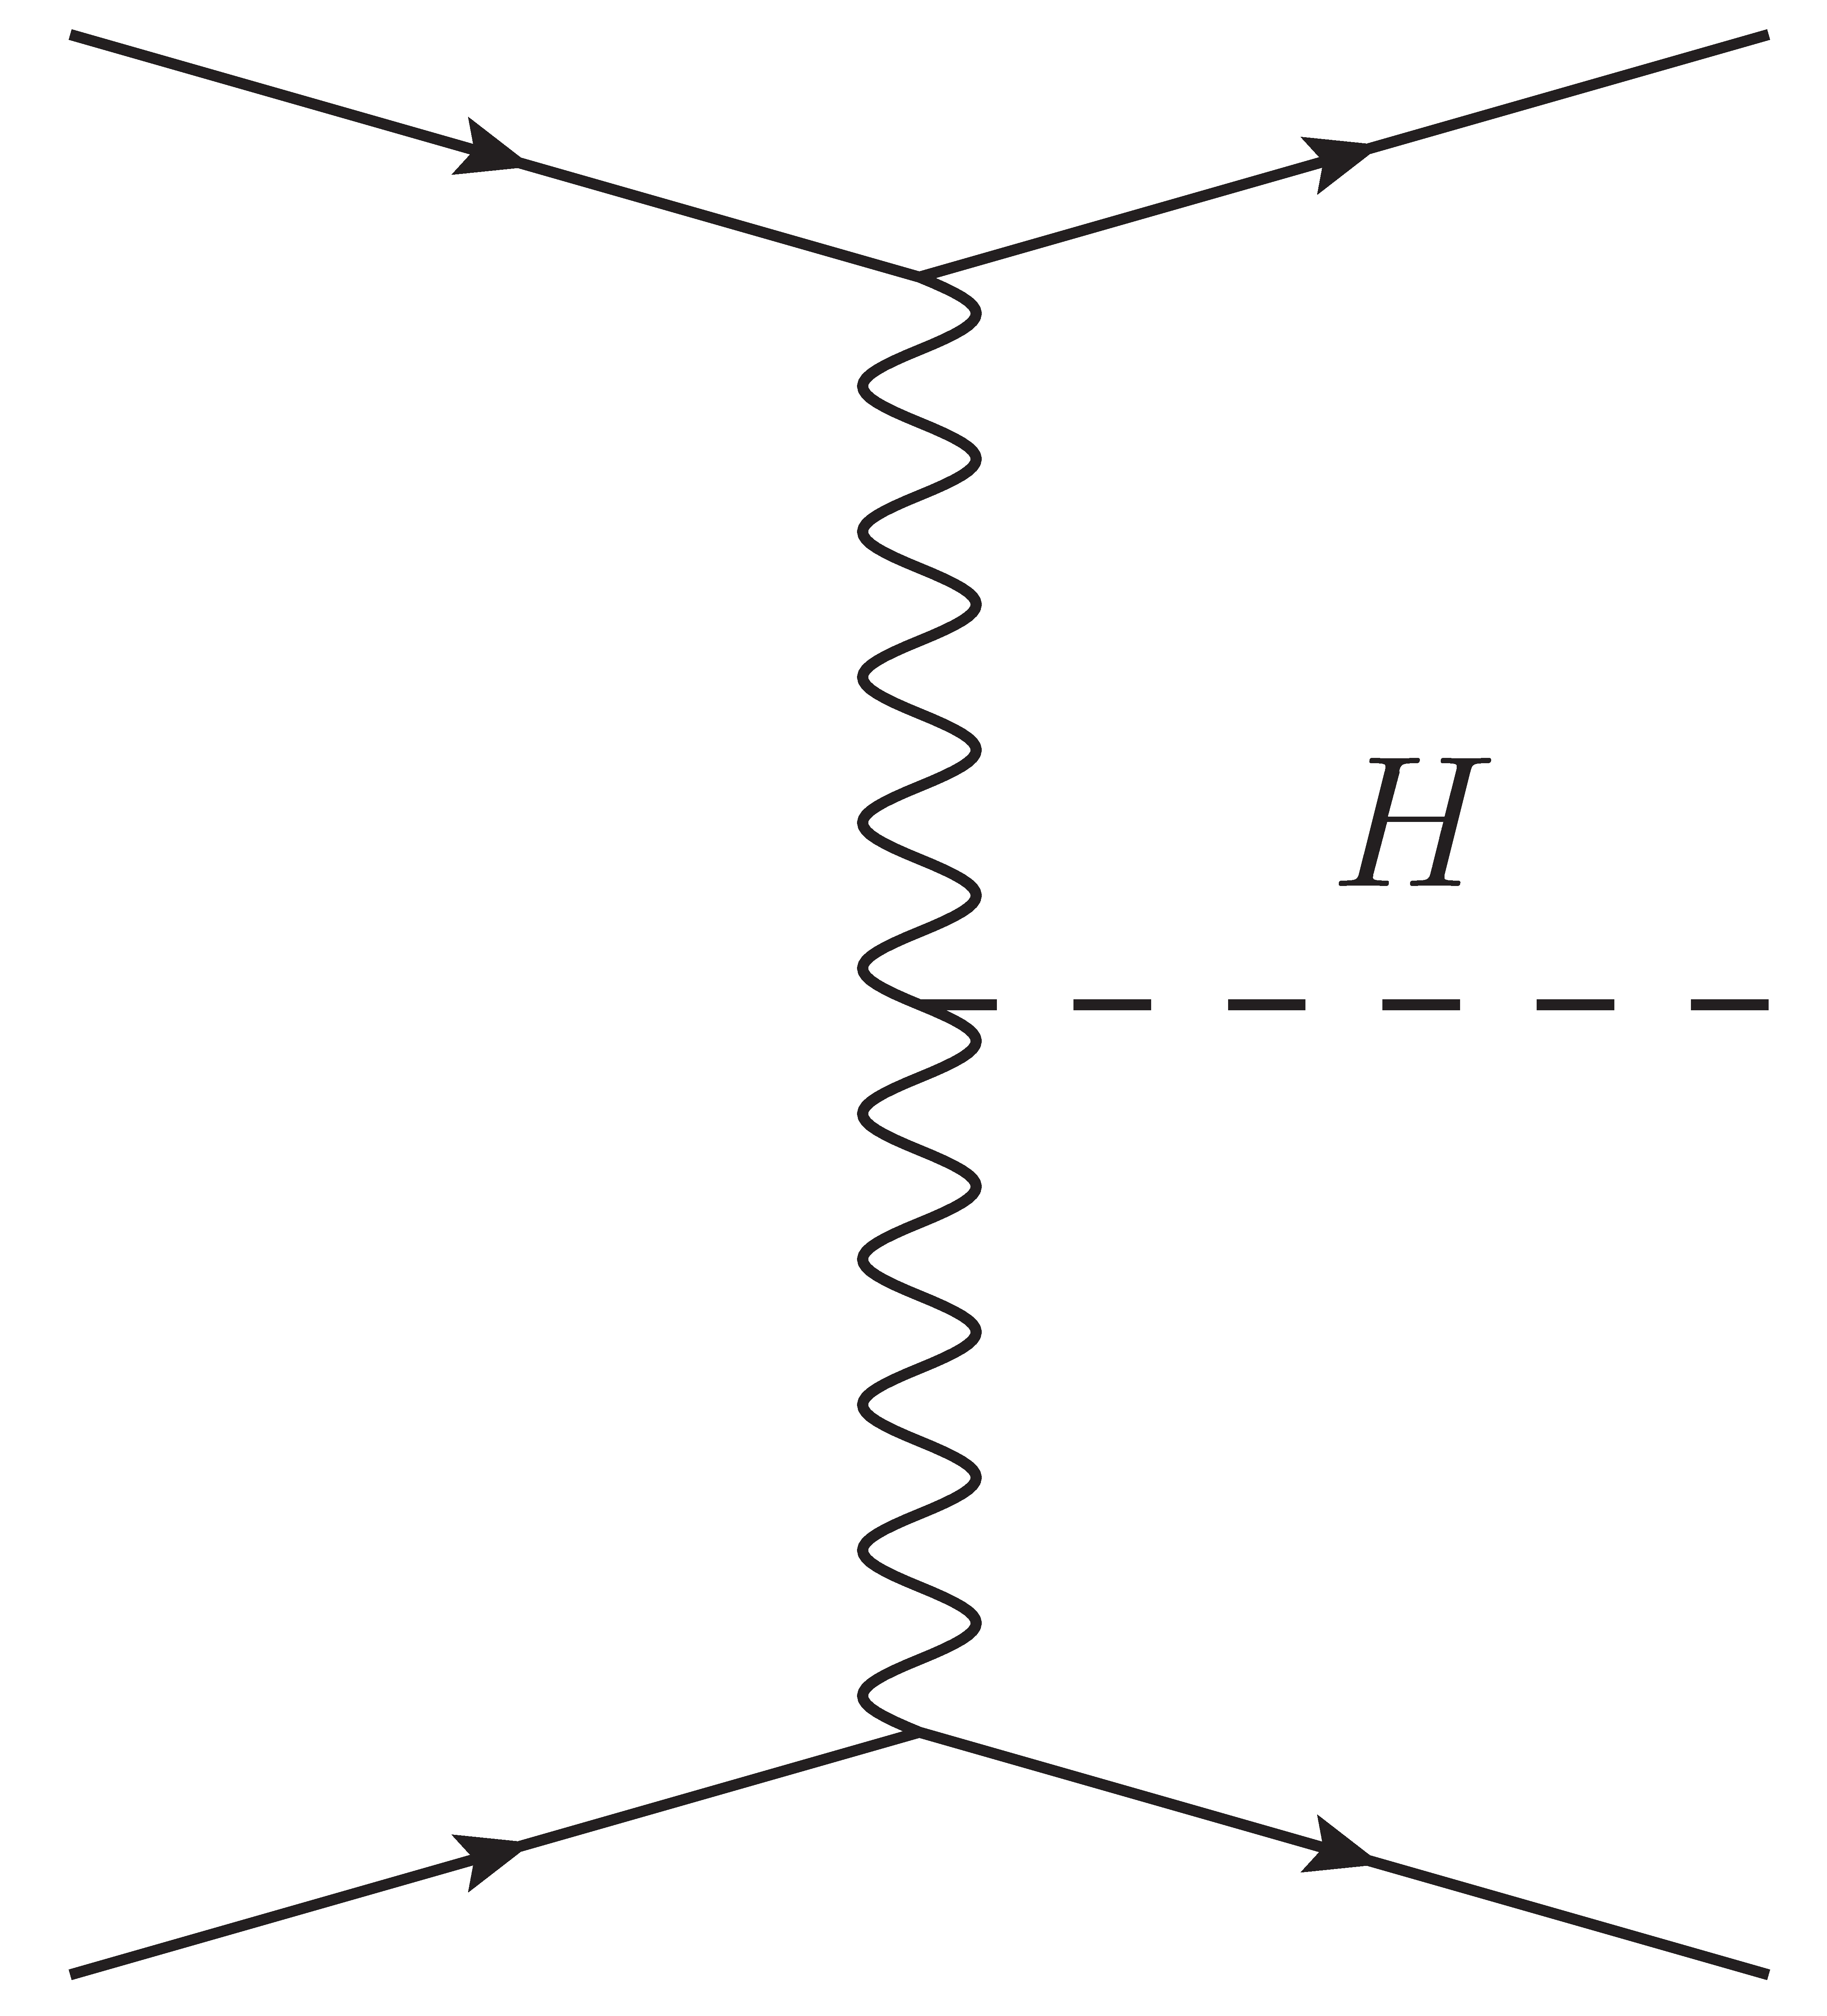
\includegraphics[scale=0.45]{figs/VBF_H.png}
    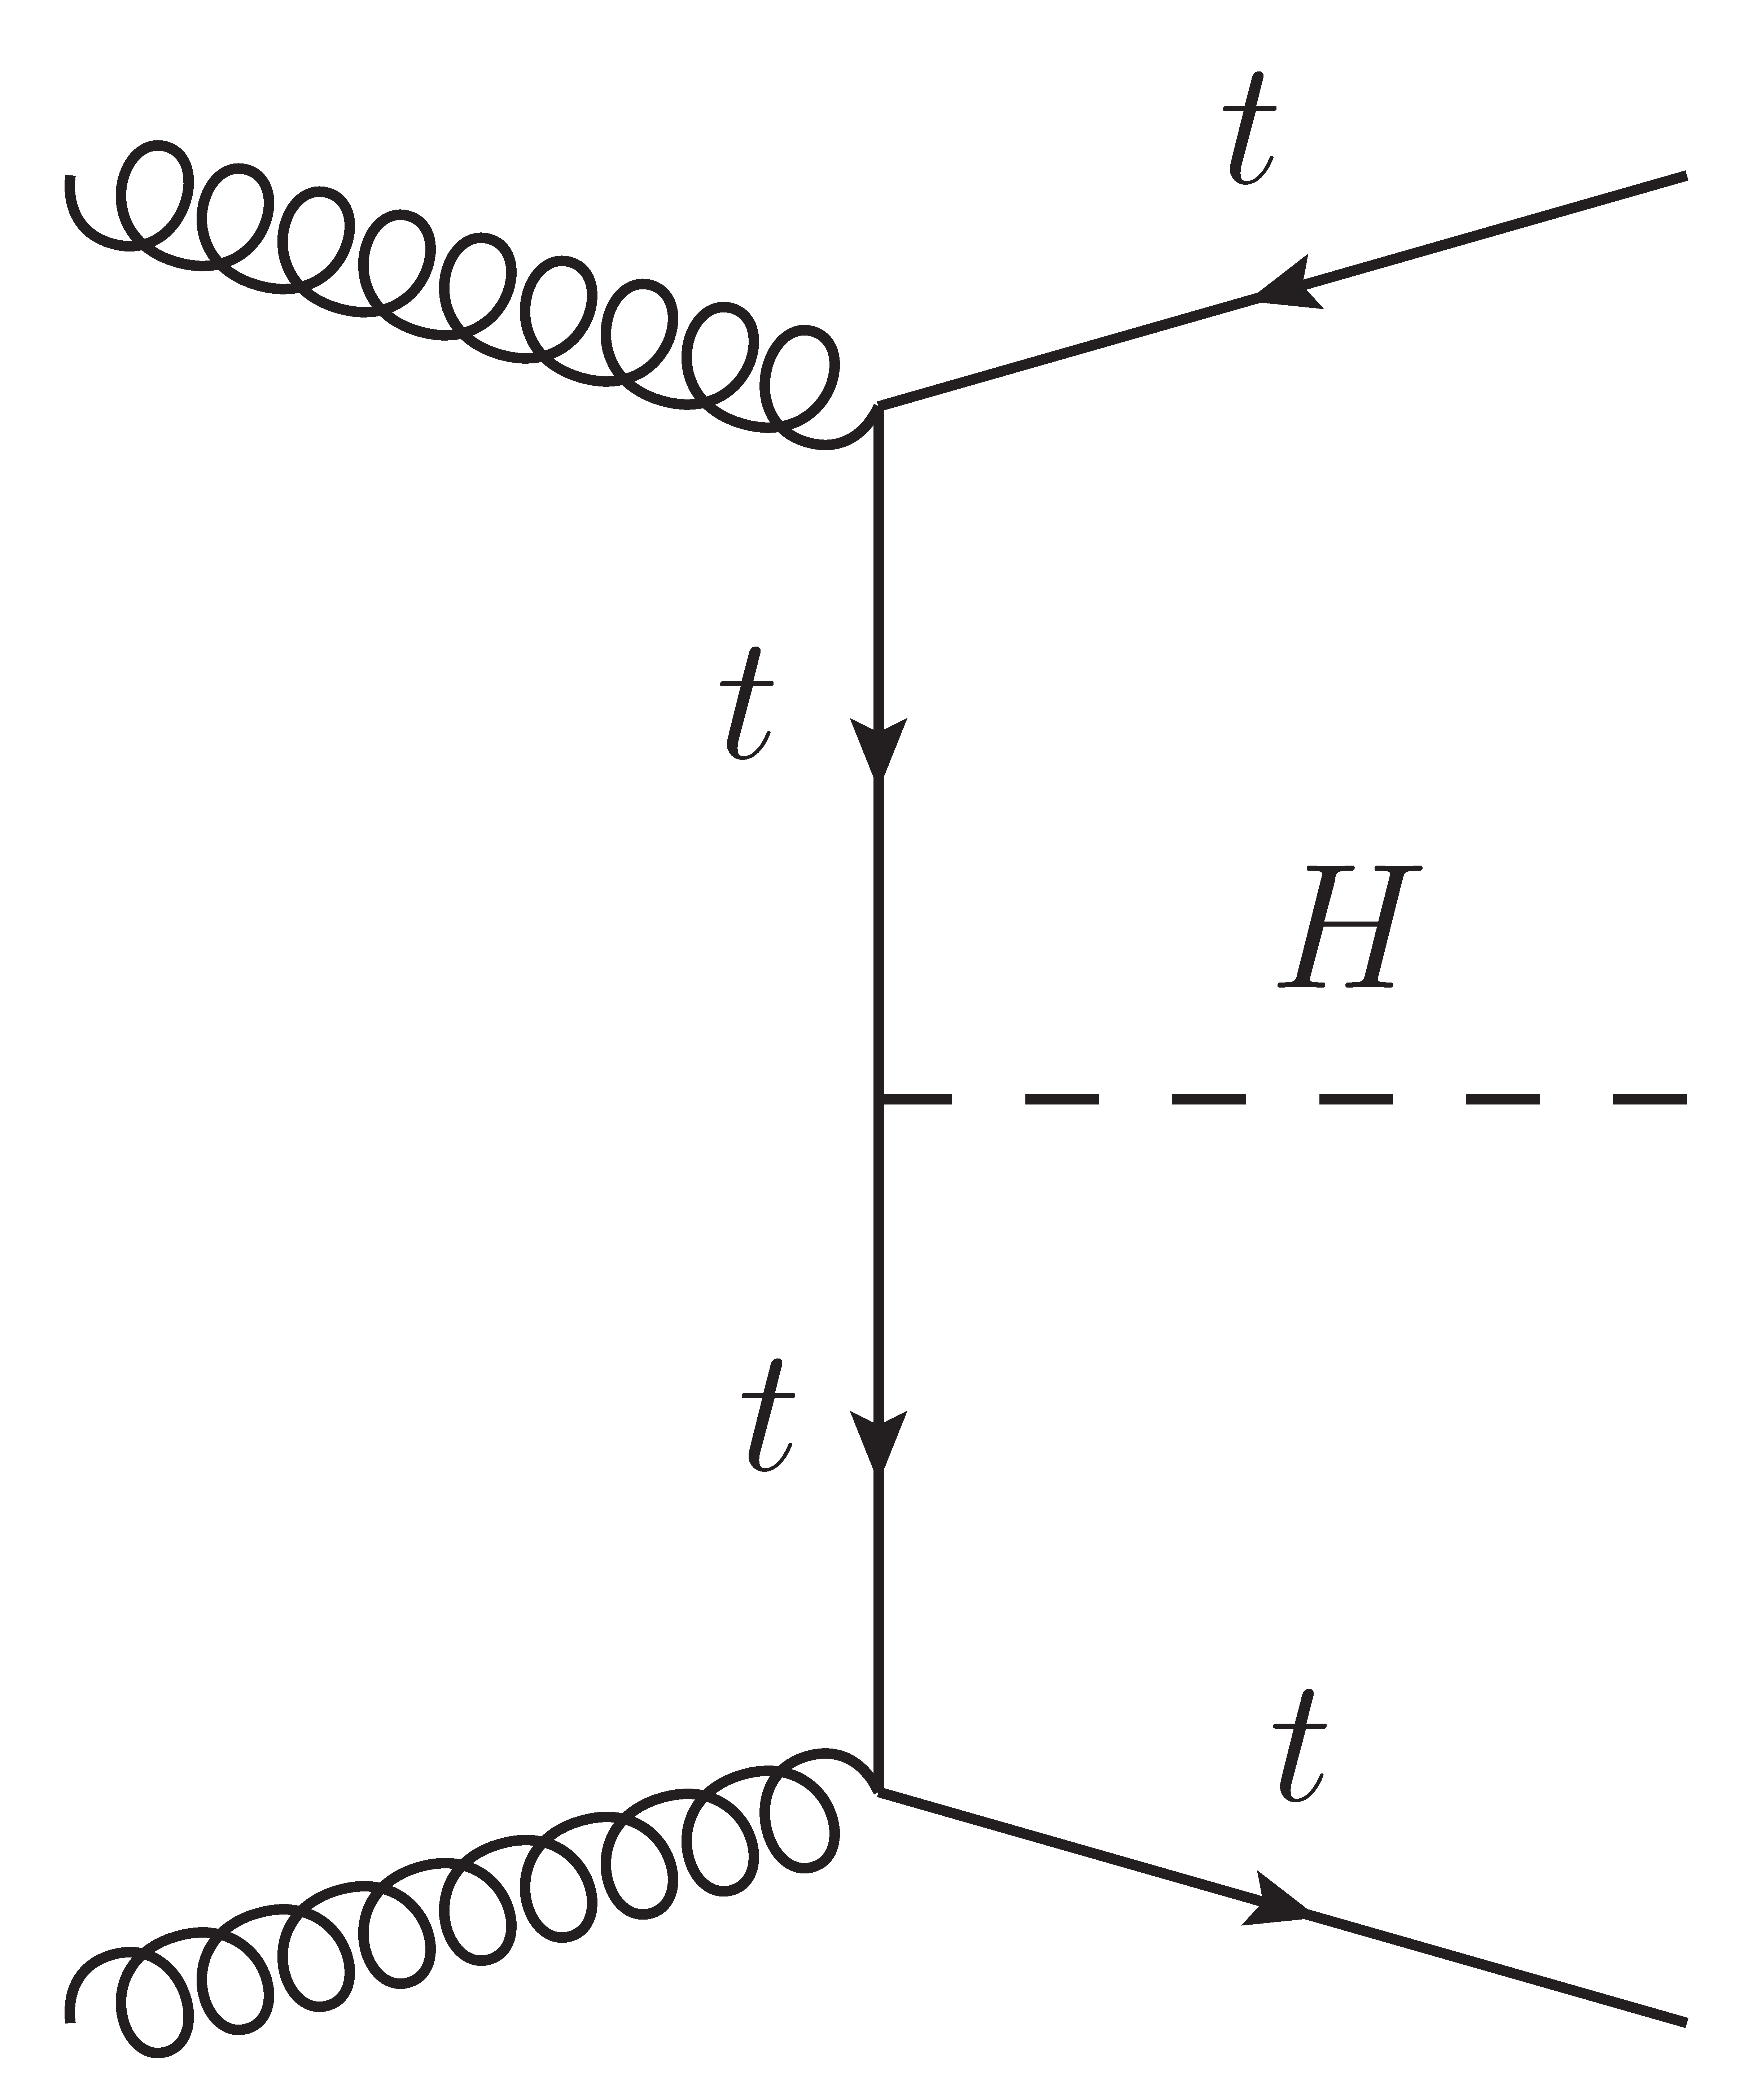
\includegraphics[scale=0.45]{figs/QuarkF_H.png}
    \caption{Higgs boson production Feynman diagrams for proton-proton collisions: gluon fusion [left-up], Higgsstrahlung [right-up], vector boson fusion [left-down] and quark fusion [right-down].}
    \label{fig:HiggsProd}
  \end{center}
\end{figure}

%\cite{Dittmaier:2011ti, Dittmaier:2012vm, Heinemeyer:2013tqa, HIGGSXSWG}
All these processes have different contributions to the Higgs boson production cross section. In figure~\ref{fig:HiggsProdXS}, the cross section of Higgs boson production for a Higgs mass of 125 GeV/$c^{2}$ for different center of mass energies at LHC is shown~\cite{HIGGSXSWG}. The dominant production is the gluon fusion, all the other processes cross sections are at least one order of magnitude smaller. The total Higgs boson production cross section at LHC is shown in figure~\ref{fig:TotalHiggsXS},~\cite{Dittmaier:2011ti, Dittmaier:2012vm, Heinemeyer:2013tqa, HIGGSXSWG}, as a function of its mass and for different center of mass energies. At run 1 energies, 7-8 TeV, the total production cross section is about 20 pb, while at 13 TeV it will be 2.3 times higher, reaching $\sim$50 pb. 

\begin{figure}[!Hhtbp]
  \begin{center}
    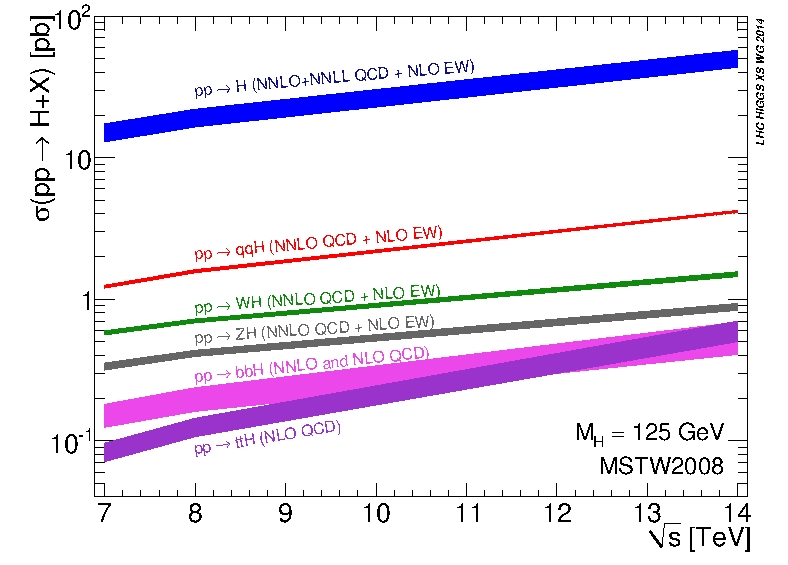
\includegraphics[width=0.6\textwidth]{figs/7-14_Higgs_xsec.jpg}
    \caption{Higgs boson theoretical production cross section as a function of center of mass energy, for a Higgs boson mass of 125 GeV/$c^{2}$~\cite{HIGGSXSWG}.}
    \label{fig:HiggsProdXS}
  \end{center}
\end{figure}

\begin{figure}[!Hhtbp]
  \begin{center}
    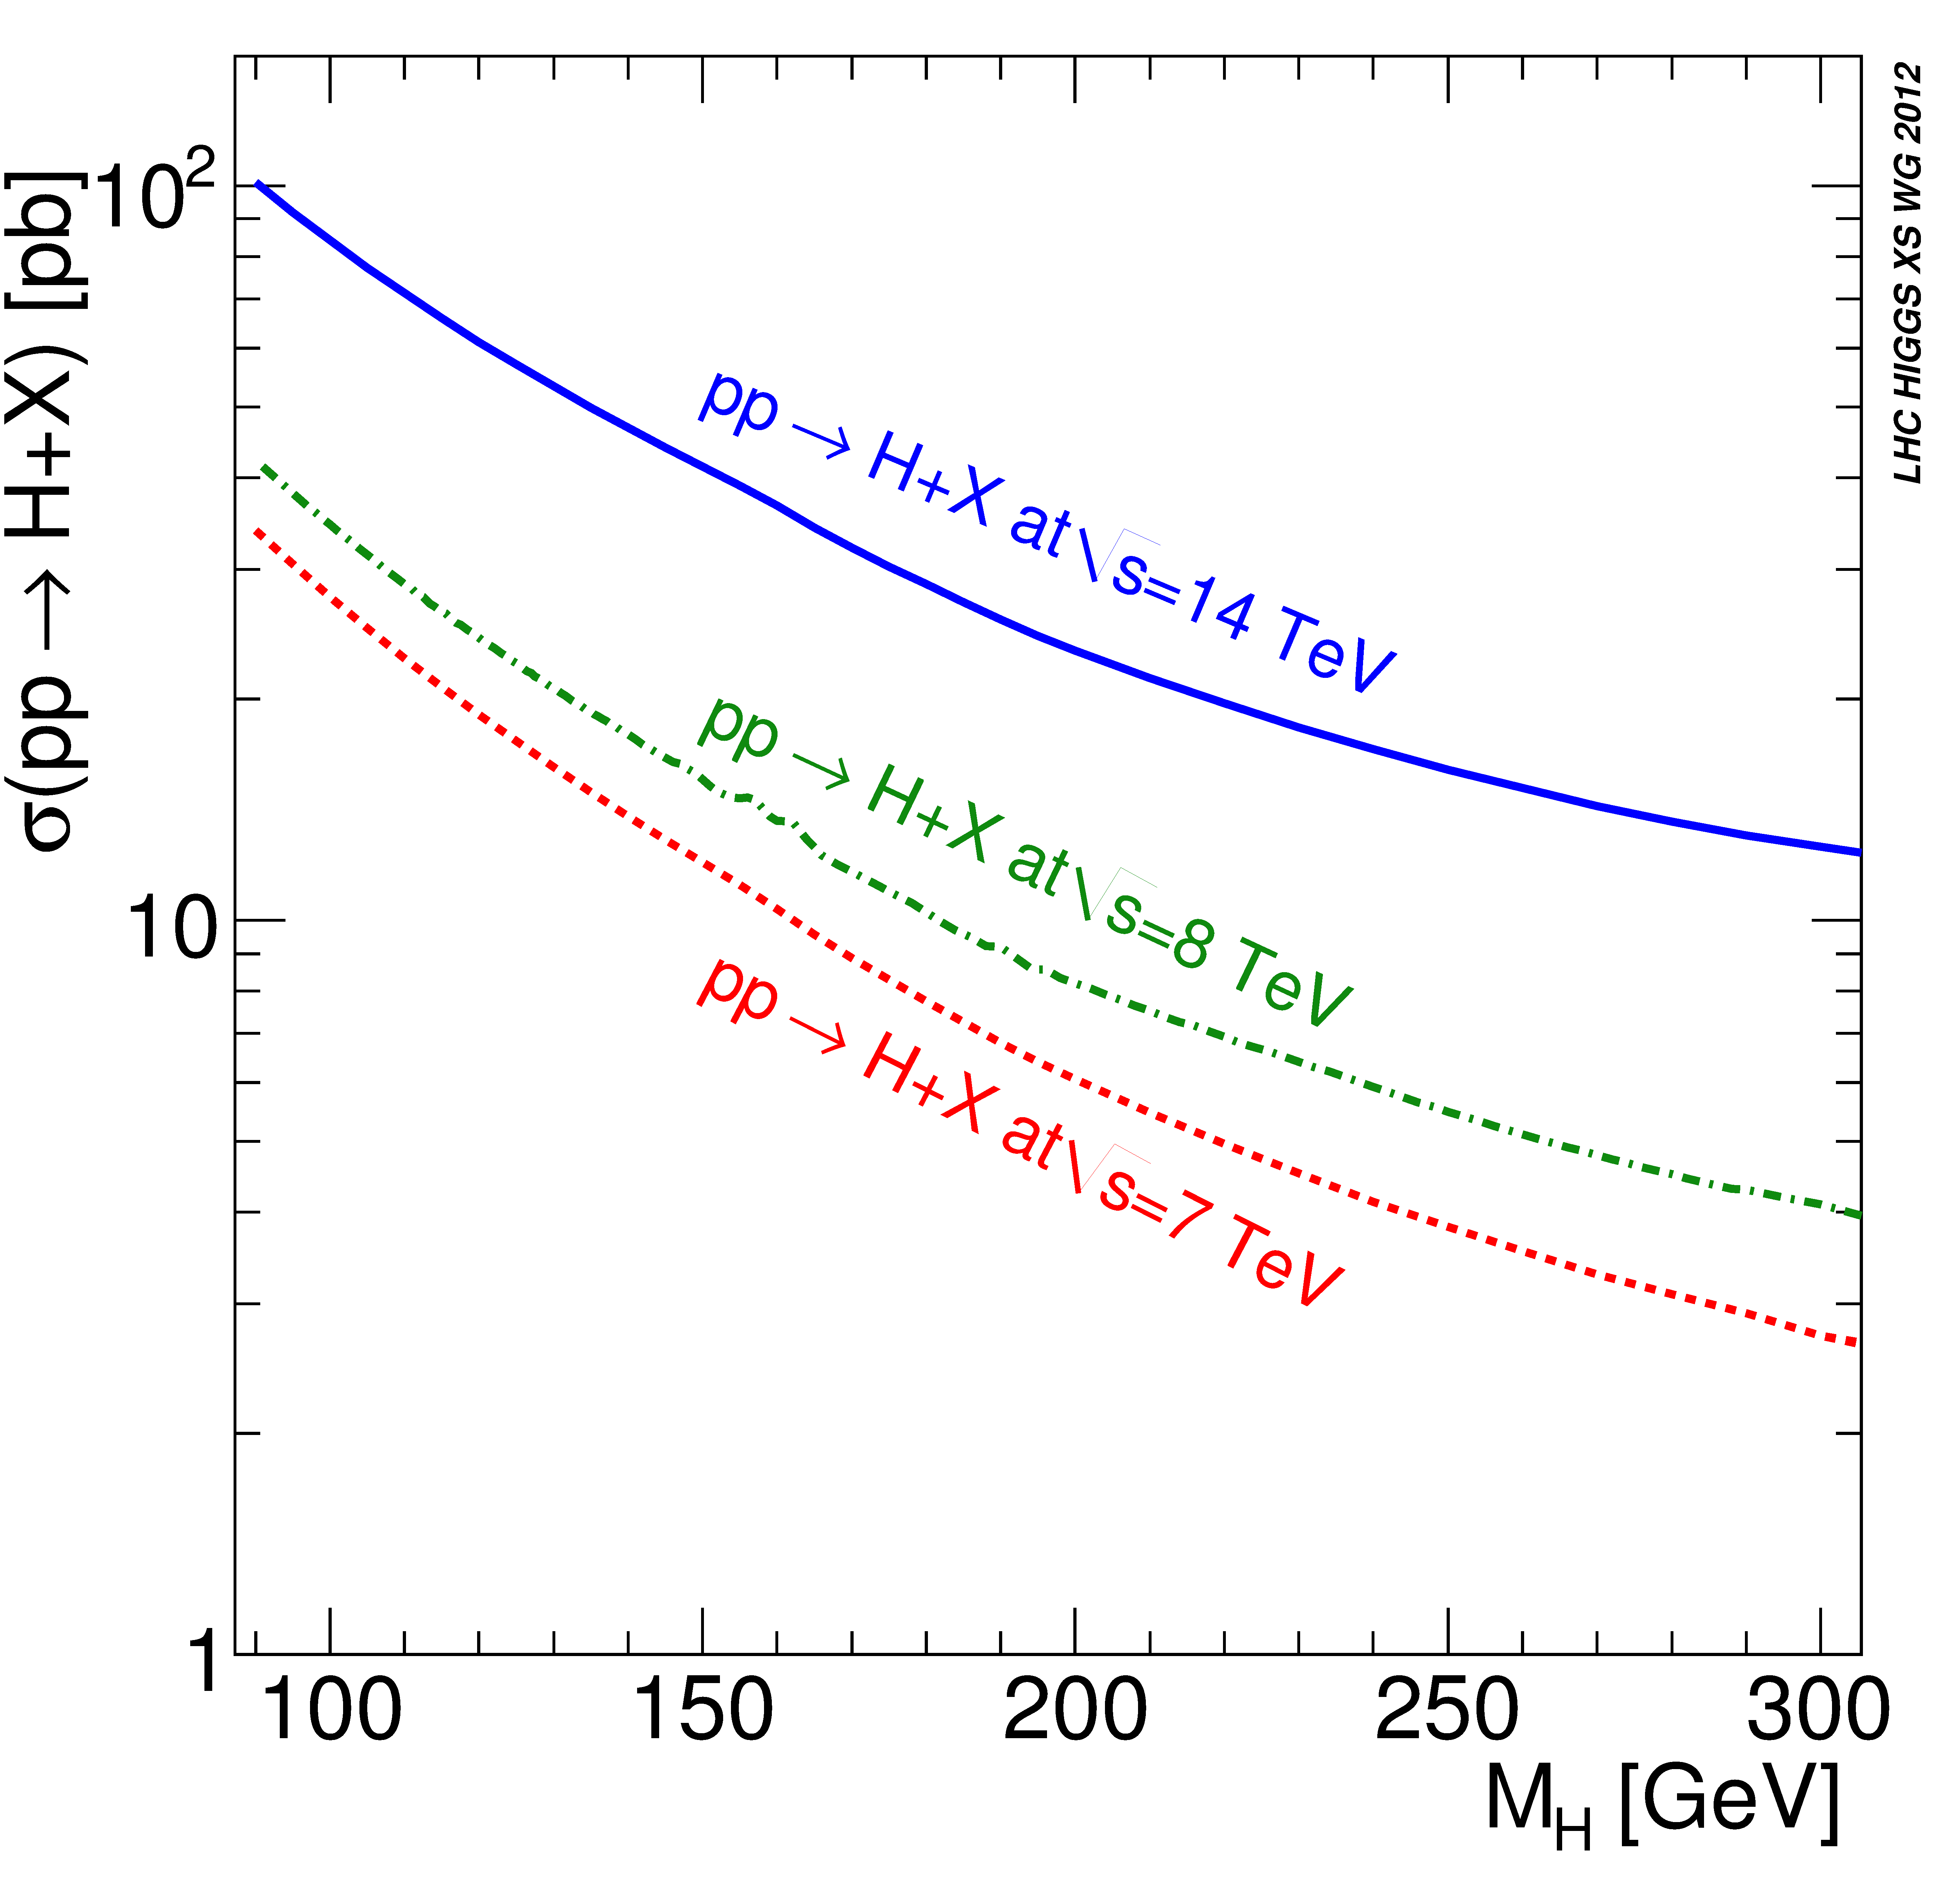
\includegraphics[width=0.6\textwidth]{figs/totalXS_LM.png}
    \caption{Total Higgs boson production cross section as a function of Higgs mass for different center of mass of proton-proton collisions~\cite{Dittmaier:2011ti, Dittmaier:2012vm, Heinemeyer:2013tqa, HIGGSXSWG}.}
    \label{fig:TotalHiggsXS}
  \end{center}
\end{figure}

%\begin{TOINCLUDE}Plots of cross section of Higgs production as a function of center of mass energy; Feynman diagrams for Higgs production\end{TOINCLUDE}

\subsection{Higgs decay channels}

As the Higgs boson couples to all particles in the SM it can decay of several ways. Figure~\ref{fig:HiggsBrs}, taken from~\cite{Dittmaier:2011ti, Dittmaier:2012vm, Heinemeyer:2013tqa, HIGGSXSWG}, shows the branching ratios of the decay channels of the Higgs boson as a function of the its mass. The highest branching ratio corresponds to its decay to two b-quarks. This channels is difficult to observe due to the high QCD and \ttbar~backgrounds, however it gives the highest expected number of events as more than the half of Higgs bosons produced at LHC decay into \bbbar~final state. The Higgs boson decay to $Z^{0}Z^{0}$ is an important channel because it has a high branching ratio and one of its final states is 4 leptons, a very clean final state (low background rate), called the golden channel. Finally, even if the diphoton channel has specially low branching ratio it is very clean in terms of photon identification and resolution. In the search that is going to be presented in chapter~\ref{chap:search}, the Higgs boson is going to be looked for in the \bbbar~decay. In figure~\ref{fig:HiggsDecays} the Feynman diagrams of the discussed decay channels are presented.

\begin{figure}[!Hhtbp]
  \begin{center}
    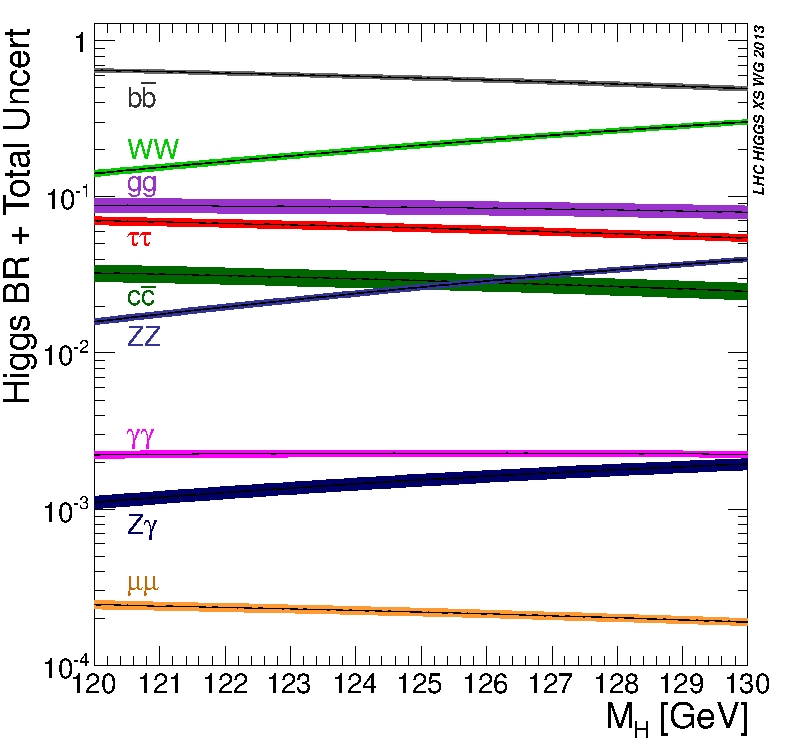
\includegraphics[width=0.8\textwidth]{figs/Higgs_BR_120-130.jpg}
    \caption{Higgs boson decay branching ratios as a function of its mass~\cite{Dittmaier:2011ti, Dittmaier:2012vm, Heinemeyer:2013tqa, HIGGSXSWG}.}
    \label{fig:HiggsBrs}
  \end{center}
\end{figure}

\begin{figure}[!Hhtbp]
  \begin{center}
    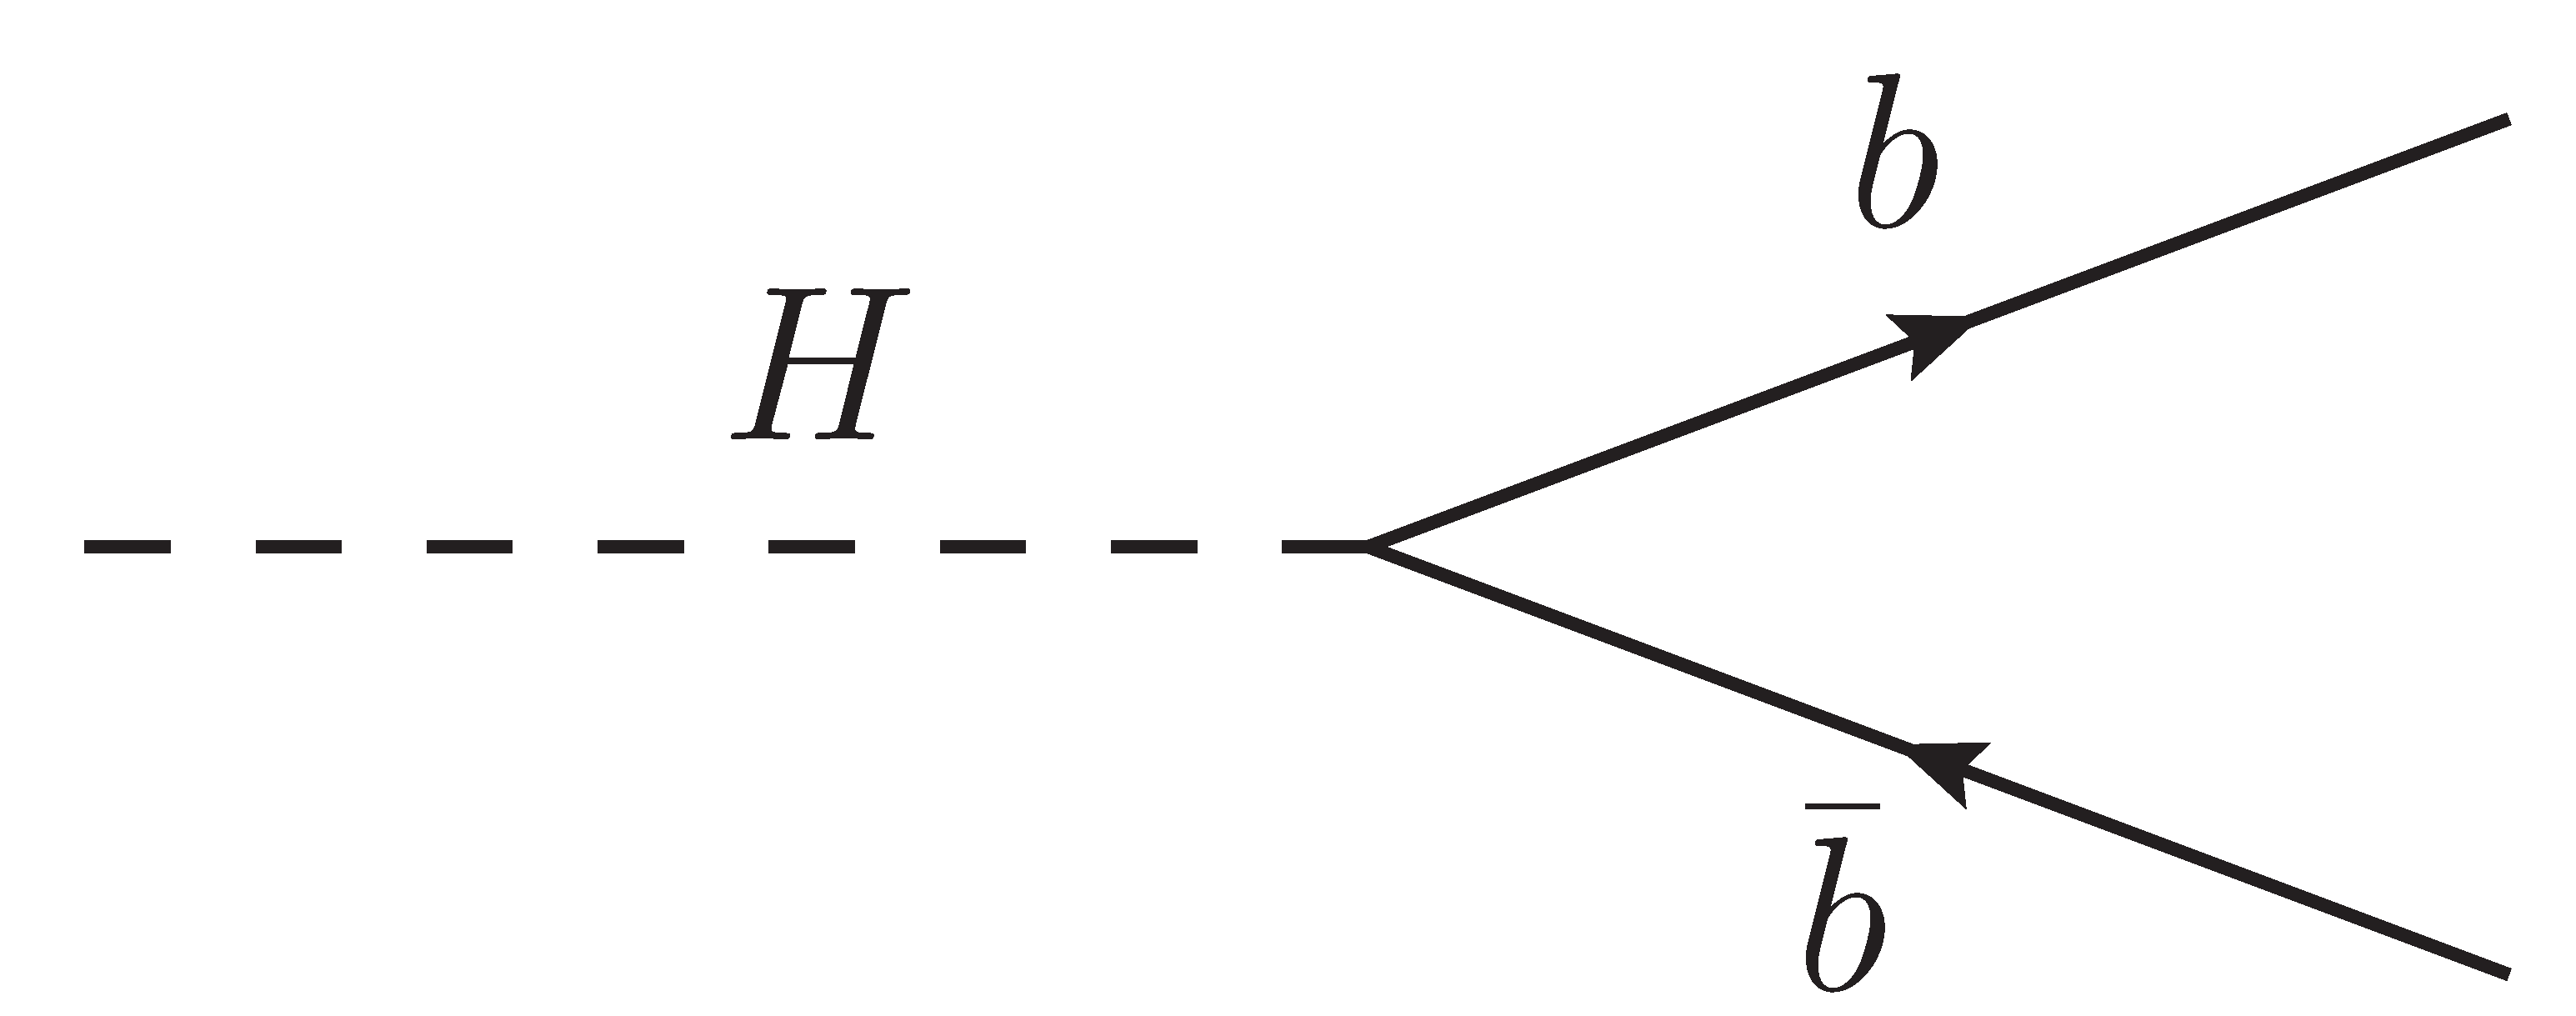
\includegraphics[width=0.3\textwidth]{figs/BB_H.png}
    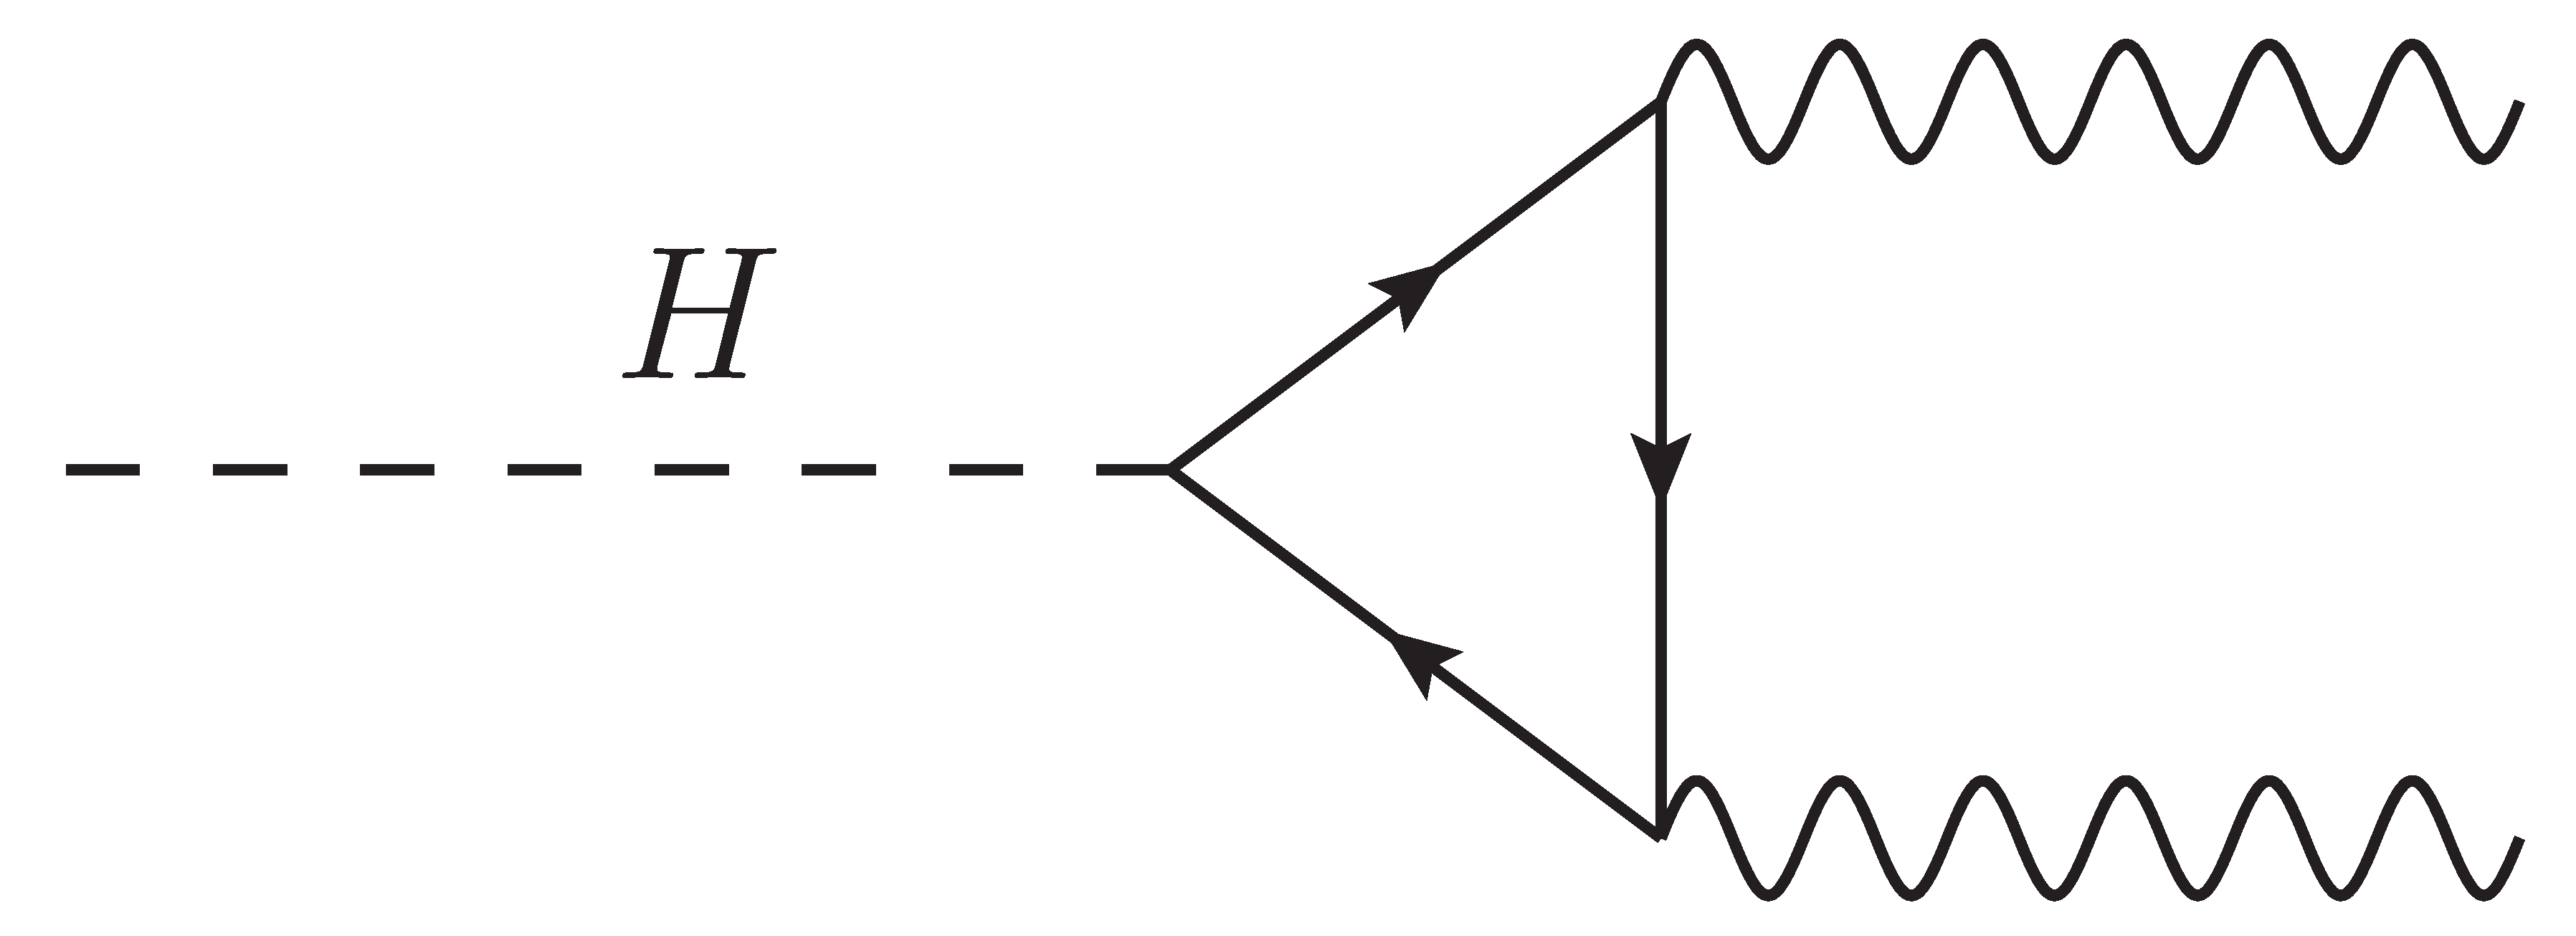
\includegraphics[width=0.3\textwidth]{figs/Diphoton_H.png}
    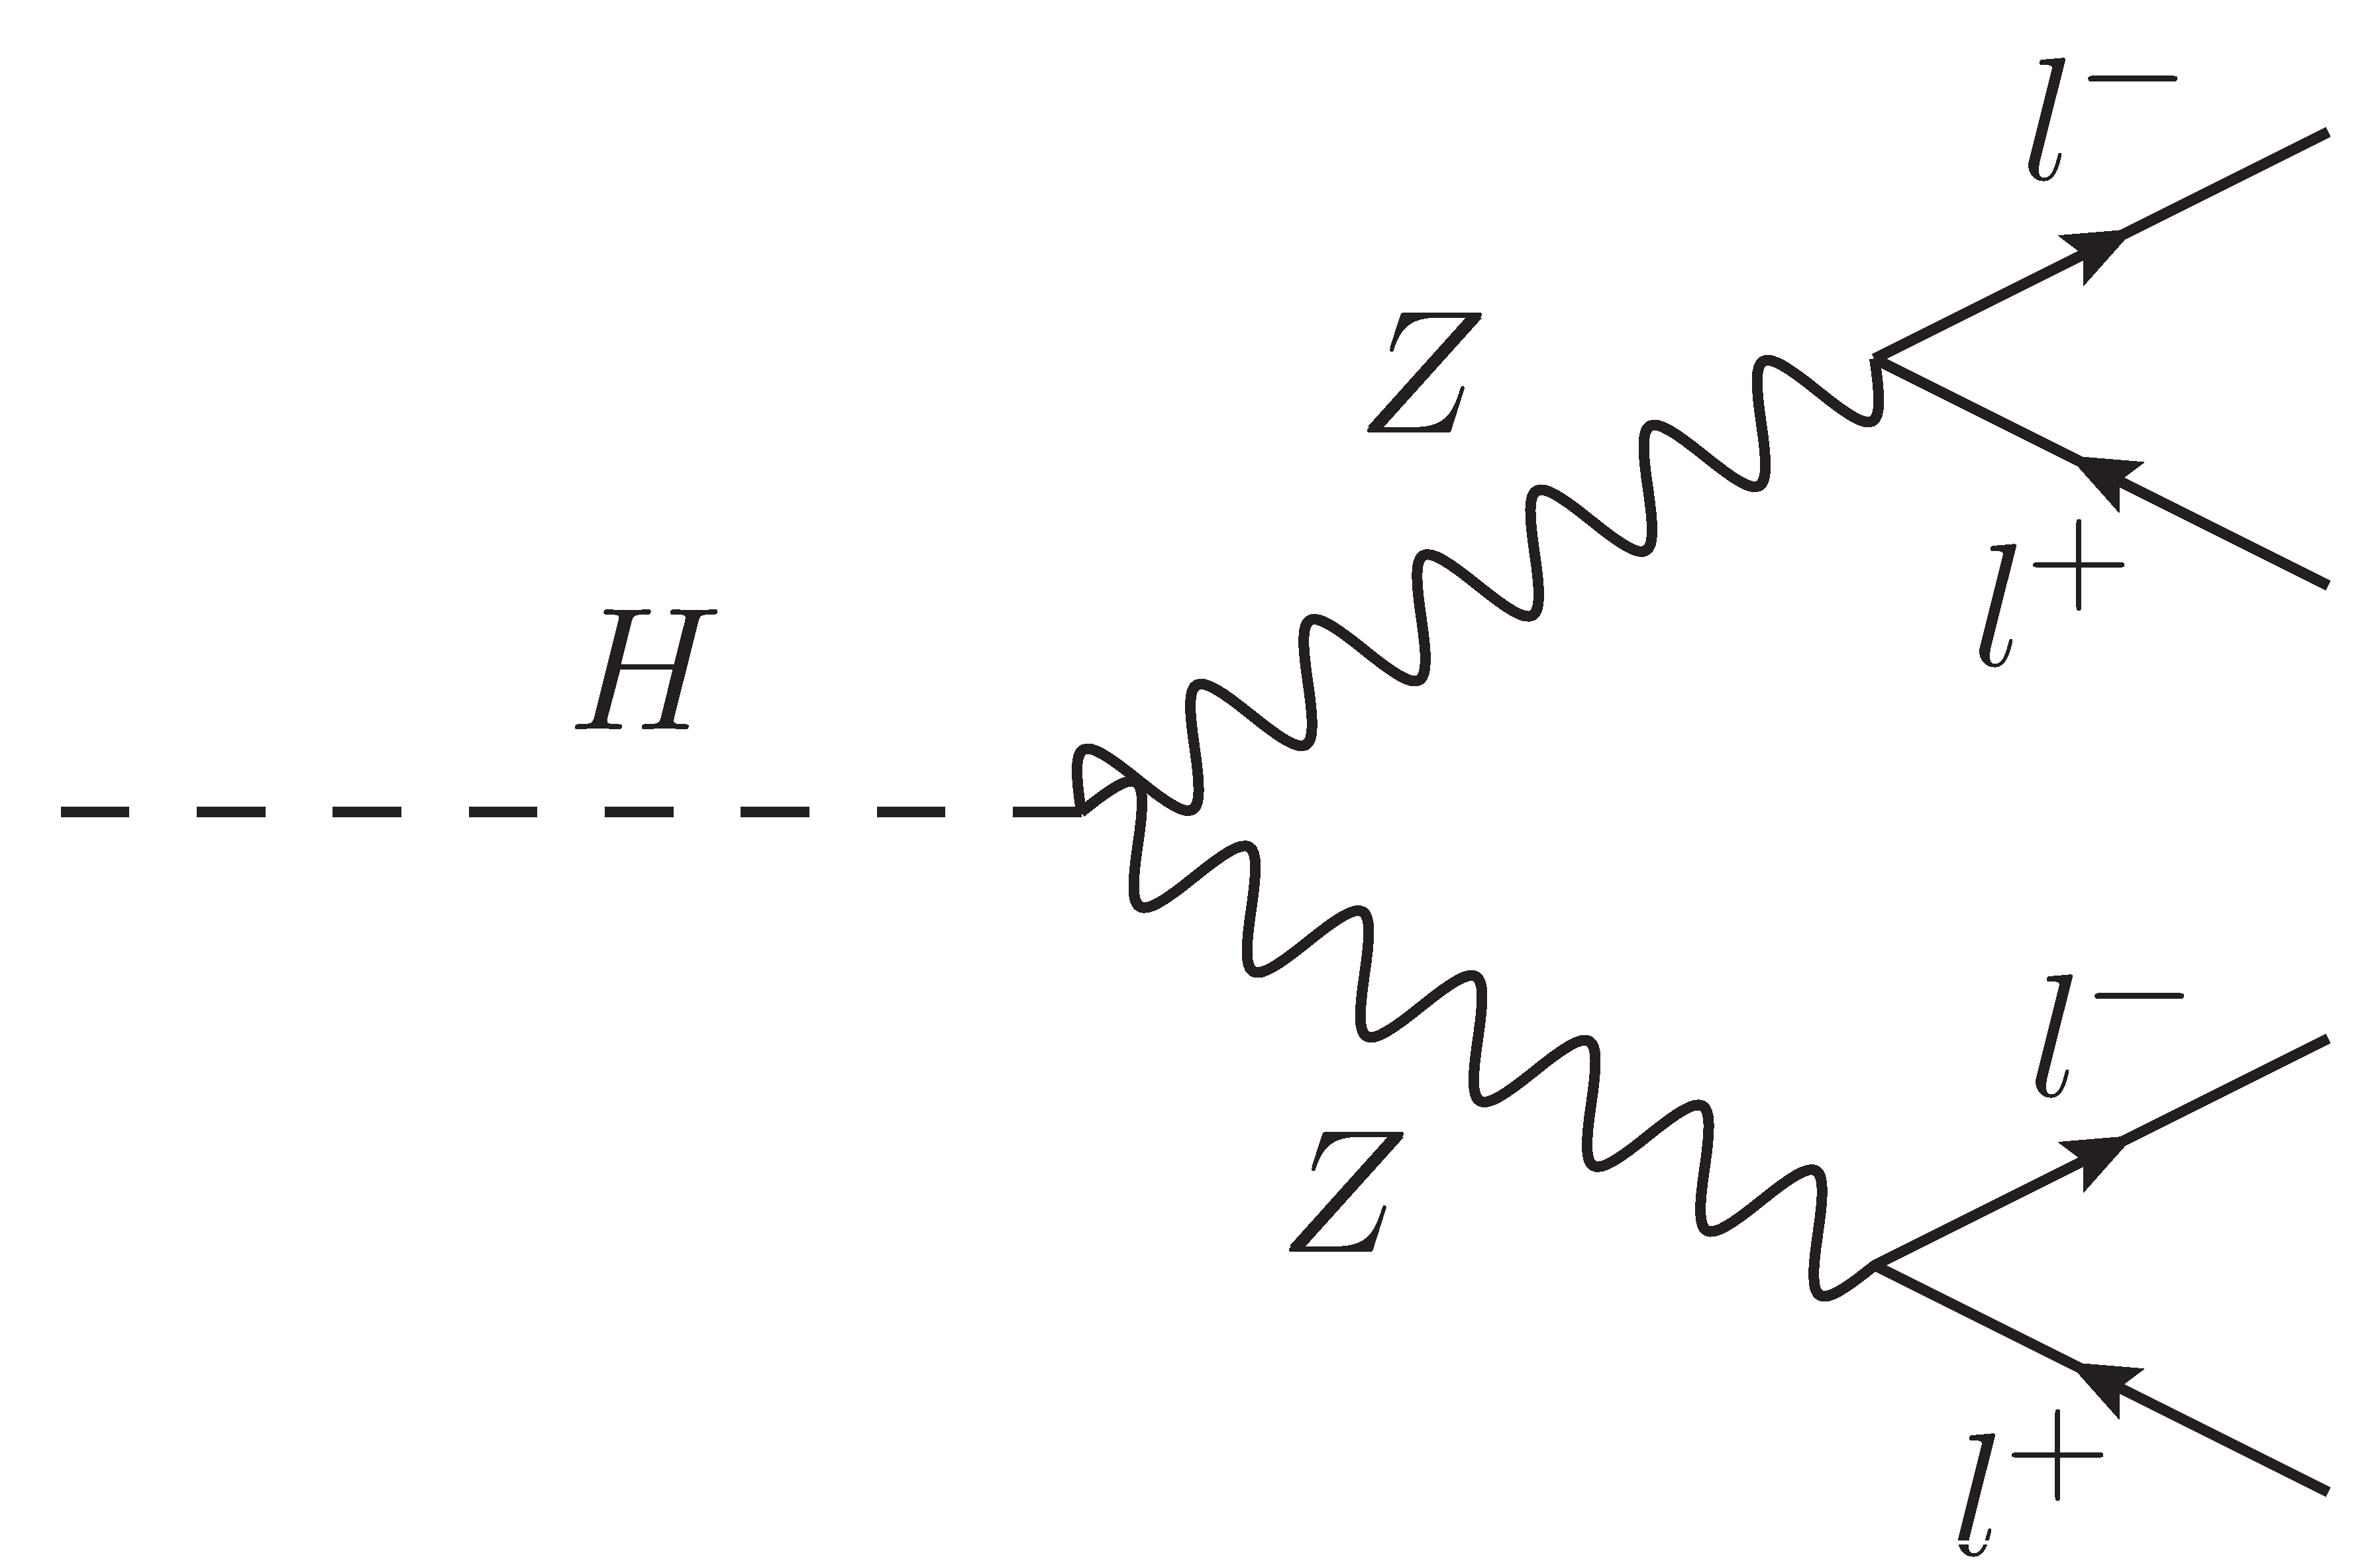
\includegraphics[width=0.3\textwidth]{figs/Golden_H.png}
    \caption{Feynman diagrams of Higgs boson decay: $b\bar{b}$ [left], diphoton [center] and golden channels [right].}
    \label{fig:HiggsDecays}
  \end{center}
\end{figure}
%\begin{TOINCLUDE}Plot on possible decay channels and branching ratios to each channel; Feynman diagram for each golden bb and diphoton channels\end{TOINCLUDE}

\subsection{Mass and width of Higgs boson}

The 4th of July of 2012 was announced the discovery of a Higgs boson like particle at LHC by ATLAS and CMS collaborations. It was discovered in several decay modes, but the most significant result was coming from the combination of results in all analyzed channels. Such searches have been refined during last years, consolidating the discovery. 

To measure the mass of the Higgs boson, diphoton and golden channel analyses have been combined between ATLAS and CMS~\cite{Aad:2015zhl}. The found value by the combination is $m_{H}=125.09\pm 0.24$. Combination and separated ATLAS and CMS results are shown in figure~\ref{fig:HiggsMass}~\cite{Aad:2015zhl,CMS:2014ega,ATLAS-CONF-2015-007}. In the same figure are shown the results, in terms of measured cross section, of all analyses done by CMS looking for a Higgs boson in different final states. The results are compatible with SM expectations.

\begin{figure}[!Hhtbp]
  \begin{center}
    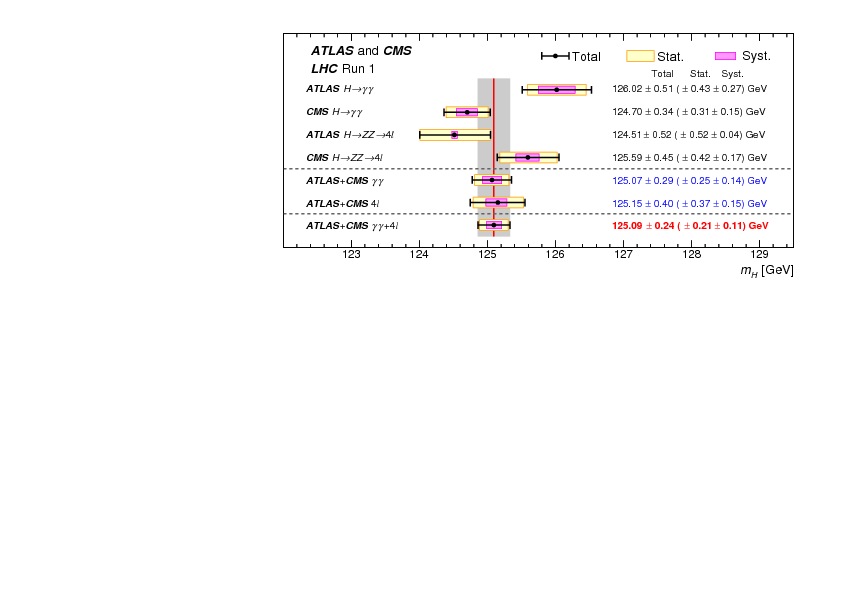
\includegraphics[trim=10cm 7cm 1cm 1cm, clip=true, width=0.8\textwidth]{figs/LHC_combined_obs_unblind_summary_a1_final.png}
    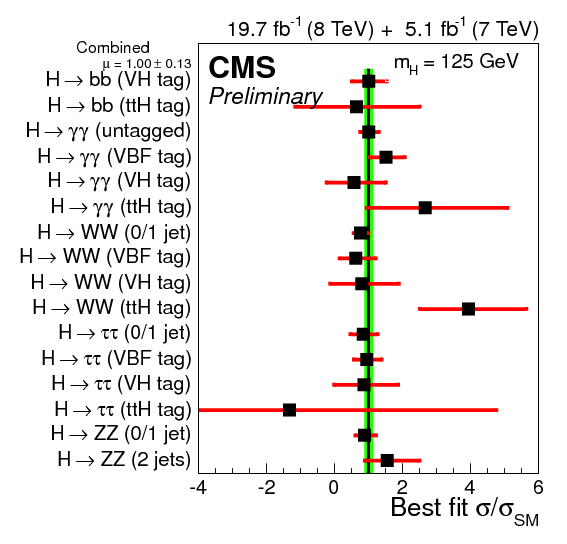
\includegraphics[width=0.55\textwidth]{figs/sqr_mlz_ccc_mH125.png}
    \includegraphics[width=0.4\textwidth]{figs/ATLAS_HIGGS_mu_Summary.png}
    \caption{ATLAS and CMS combination of Higgs boson mass measurement [top] and $\sigma/\sigma_{SM}$ (measured cross section over theoretical SM cross section) for searches performed by ATLAS and CMS in different Higgs boson decay channels [bottom]~\cite{Aad:2015zhl,CMS:2014ega,ATLAS-CONF-2015-007}.}
    \label{fig:HiggsMass}
  \end{center}
\end{figure}

Whereas nowadays there are plenty of experimental results for the measurement of Higgs boson mass, measuring the Higgs boson width constitutes an important challenge. The predicted width from the SM is $\sim$4 MeV for a 125 GeV mass Higgs. Figure~\ref{fig:WidthHiggs} shows the width dependence on the Higgs boson mass, taken from~\cite{Dittmaier:2011ti, Dittmaier:2012vm, Heinemeyer:2013tqa, HIGGSXSWG}. In the same figure is shown a method proposed by CMS collaboration using the golden channel to constraint Higgs boson width~\cite{Khachatryan:2014iha}. Such method put a limit of about 4.2 times the SM Higgs width ($\sim$20 MeV).

\begin{figure}[!Hhtbp]
  \begin{center}
    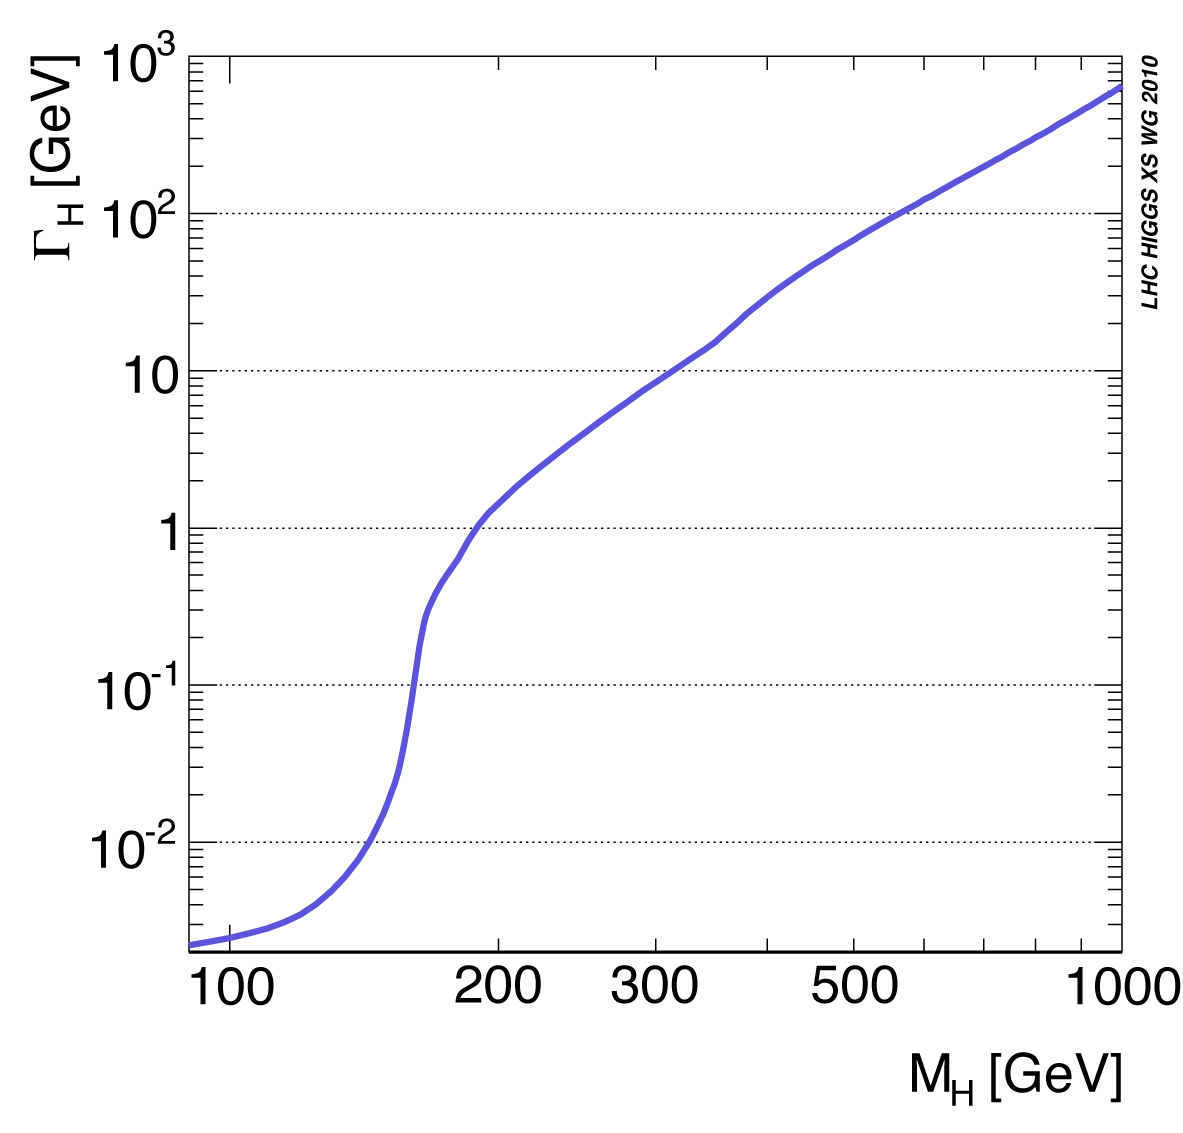
\includegraphics[width=0.42\textwidth]{figs/u0g5o.png}
    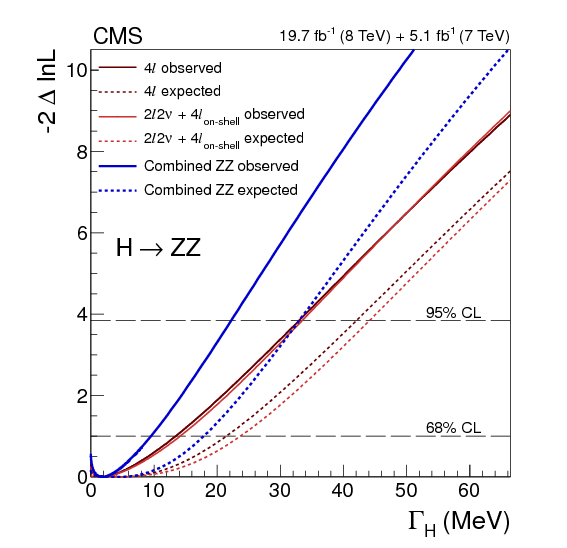
\includegraphics[width=0.42\textwidth]{figs/AllFitPaper_30_04_14_MeV.png}
    \caption{Higgs boson width as a function of its mass~\cite{Dittmaier:2011ti, Dittmaier:2012vm, Heinemeyer:2013tqa, HIGGSXSWG} [left] and current limits from CMS measurement~\cite{Khachatryan:2014iha} [right].}
    \label{fig:WidthHiggs}
  \end{center}
\end{figure}

%\begin{figure}[!Hhtbp]
%  \begin{center}
%    
\includegraphics[width=0.3\textwidth]{figs/CMSlogo.png}
%    \caption{}
%    \label{fig:}
%  \end{center}
%\end{figure}
%\begin{TOINCLUDE}Plot on ATLAS+CMS combination of the Higgs mass; Plot on signal strength for each decay channel; Individual plots on diphoton channel and golden channel\end{TOINCLUDE}


%\begin{TOINCLUDE}Plot of branching ratio as a function of the mass for different scenarios (representations)\end{TOINCLUDE}

